

\input{../Latex_Templates/Preamble_Report}

%%%%% TITLE PAGE

%\subject{, VT23}
\title{ Report for the Course Modelling in Computational Science, HT23 \\[1ex]
	  \large Project 1: The Potts model}
%\subtitle{}
\author{Theo Koppenhöfer}
\date{Lund \\[1ex] \today}

\addbibresource{bibliography.bib}

\usepackage{pythonhighlight}
\usepackage{pgfplots}
\graphicspath{{../Figures/}}

\pgfplotsset{compat=newest,
    width=10cm,
    height=10cm,
    max space between ticks=25pt,
    try min ticks=5,
    every axis/.style={
        axis y line=left,
        axis x line=bottom,
        axis line style={thick,->,>=latex, shorten >=-.4cm}
    },
    every axis plot/.append style={thick},
    tick style={black, thick}
}

%%%%% The content starts here %%%%%%%%%%%%%


\begin{document}

\maketitle

\section{Introduction}

The following report is part of the first project of the Modelling in Computational Science course at Lund University, HT2023.
In the first project we implemented a Monte-Carlo simulation of the $q$-state Potts model.
The report and the Python implementation can be found online under \cite{Repository}

\section{The Potts model}

A state of the $q$-state Potts model of a $L\times L$ flat grid is given by a mapping
\begin{align*}
	s\colon \brk[c]{1,\dots,L}\times\brk[c]{1,\dots,L}\to\brk[c]{1,\dots,L}\,.
\end{align*}
One assigns this state an energy via
\begin{align*}
	E = -J\sum_{\substack{i, j\text{ neighbouring}\\ \text{grid points}}}\delta\brk*{s_i,s_j}
\end{align*}
where $\delta$ denotes the Kronecker-delta and $J=1$ is the coupling strength. As given in the problem setting we assume periodic boundary conditions on the grid.

\section{The implementation}

\subsubsection{Determining when the Energy has plateaued}

The energy of the system takes some time $t_0$ to reach an equilibrium state. To determine $t_0$ we calculate in every step $i$ moving averages $\text{ma}_1$ and $\text{ma}_2$ over $n$ energies. The construction is shown in figure \ref{fi:movingAverages}. If we start in the hot state then the energy will tend to shrink until we reach an equilibrium. Hence we can use the condition
\begin{align}
	\text{ma}_2 \leq \text{ma}_1 \label{eq:equilCondition}
\end{align}
to determine $t_0$. If on the other hand we start in cold state the energy will in general increase and we have to reverse the inequality in equation \eqref{eq:equilCondition}. After reaching an equilibrium the simulation runs for a further \pyth{M_sampling=5000} steps. It is over these samples we take the mean and the variance.

\begin{figure}
\centering
\input{../Figures/explanationMovingAverages.pdf_tex}
\caption{Explanation of the moving averages.}
\label{fi:movingAverages}
\end{figure}

\subsubsection{Improving performance}
While simulating we run into performance issues due to the fact that Python is in general rather slow even with heavy use of Numpy. We resolved this issue with the help of Numba which precompiled functions and thus increased performance substantially. The downside is that the code becomes quite unestetic because Numba only supports some Python and Numpy features. We noted during the simulation of the 


\begin{figure}
\centering
% This file was created with tikzplotlib v0.10.1.
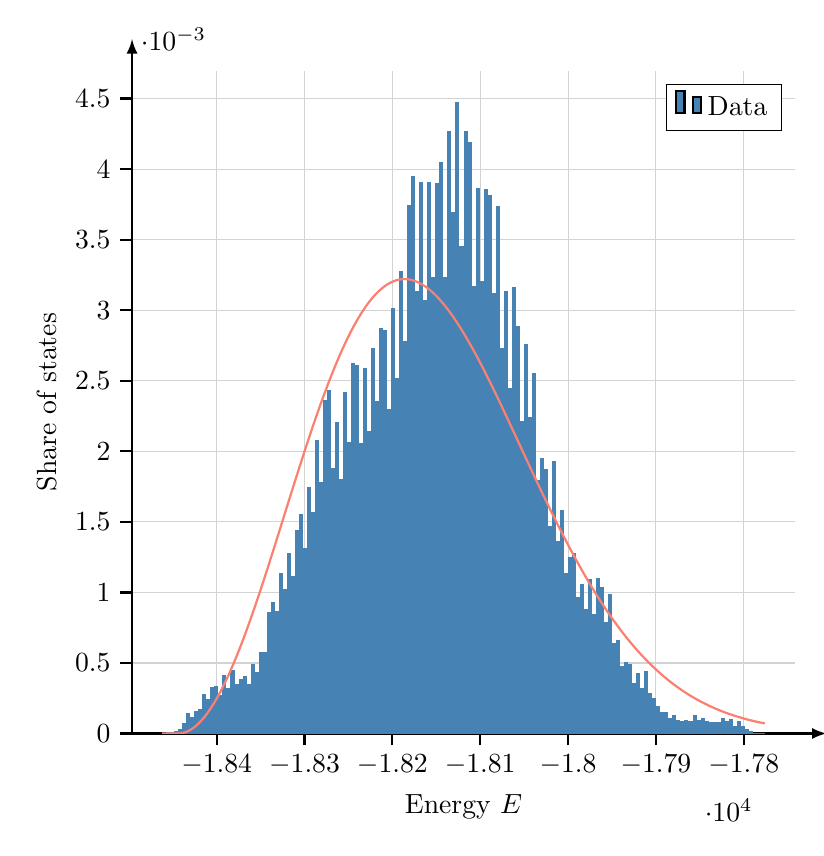
\begin{tikzpicture}

\definecolor{lightgray}{RGB}{211,211,211}
\definecolor{salmon}{RGB}{250,128,114}
\definecolor{steelblue}{RGB}{70,130,180}

\begin{axis}[
tick align=outside,
tick pos=left,
x grid style={lightgray},
xlabel={Energy \(\displaystyle E\)},
xmajorgrids,
xmin=-18496.3, xmax=-17741.7,
xtick style={color=black},
y grid style={lightgray},
ylabel={Share of states},
ymajorgrids,
ymin=0, ymax=0.00469779336734654,
ytick style={color=black}
]
\draw[draw=none,fill=steelblue] (axis cs:-18462,0) rectangle (axis cs:-18457.4266666667,5.90379008746306e-06);
\addlegendimage{ybar,ybar legend,draw=none,fill=steelblue}
\addlegendentry{Data}

\draw[draw=none,fill=steelblue] (axis cs:-18457.4266666667,0) rectangle (axis cs:-18452.8533333333,1.1752915451894e-05);
\draw[draw=none,fill=steelblue] (axis cs:-18452.8533333333,0) rectangle (axis cs:-18448.28,1.32835276967919e-05);
\draw[draw=none,fill=steelblue] (axis cs:-18448.28,0) rectangle (axis cs:-18443.7066666667,1.47048104956256e-05);
\draw[draw=none,fill=steelblue] (axis cs:-18443.7066666667,0) rectangle (axis cs:-18439.1333333333,3.29081632653295e-05);
\draw[draw=none,fill=steelblue] (axis cs:-18439.1333333333,0) rectangle (axis cs:-18434.56,7.2813411078711e-05);
\draw[draw=none,fill=steelblue] (axis cs:-18434.56,0) rectangle (axis cs:-18429.9866666667,0.00014185495626821);
\draw[draw=none,fill=steelblue] (axis cs:-18429.9866666667,0) rectangle (axis cs:-18425.4133333333,0.00011856778425655);
\draw[draw=none,fill=steelblue] (axis cs:-18425.4133333333,0) rectangle (axis cs:-18420.84,0.000156614431486867);
\draw[draw=none,fill=steelblue] (axis cs:-18420.84,0) rectangle (axis cs:-18416.2666666667,0.000177004373177828);
\draw[draw=none,fill=steelblue] (axis cs:-18416.2666666667,0) rectangle (axis cs:-18411.6933333333,0.000281031341107848);
\draw[draw=none,fill=steelblue] (axis cs:-18411.6933333333,0) rectangle (axis cs:-18407.12,0.000244241982507268);
\draw[draw=none,fill=steelblue] (axis cs:-18407.12,0) rectangle (axis cs:-18402.5466666667,0.000328152332361488);
\draw[draw=none,fill=steelblue] (axis cs:-18402.5466666667,0) rectangle (axis cs:-18397.9733333333,0.0003377186588921);
\draw[draw=none,fill=steelblue] (axis cs:-18397.9733333333,0) rectangle (axis cs:-18393.4,0.000270973032070163);
\draw[draw=none,fill=steelblue] (axis cs:-18393.4,0) rectangle (axis cs:-18388.8266666667,0.000417638483964979);
\draw[draw=none,fill=steelblue] (axis cs:-18388.8266666667,0) rectangle (axis cs:-18384.2533333333,0.000323341836734666);
\draw[draw=none,fill=steelblue] (axis cs:-18384.2533333333,0) rectangle (axis cs:-18379.68,0.000452842565597629);
\draw[draw=none,fill=steelblue] (axis cs:-18379.68,0) rectangle (axis cs:-18375.1066666667,0.000348870262390641);
\draw[draw=none,fill=steelblue] (axis cs:-18375.1066666667,0) rectangle (axis cs:-18370.5333333333,0.000382817055393553);
\draw[draw=none,fill=steelblue] (axis cs:-18370.5333333333,0) rectangle (axis cs:-18365.96,0.000406760204081598);
\draw[draw=none,fill=steelblue] (axis cs:-18365.96,0) rectangle (axis cs:-18361.3866666667,0.000353407434402302);
\draw[draw=none,fill=steelblue] (axis cs:-18361.3866666667,0) rectangle (axis cs:-18356.8133333333,0.000493841107871678);
\draw[draw=none,fill=steelblue] (axis cs:-18356.8133333333,0) rectangle (axis cs:-18352.24,0.000432780612245206);
\draw[draw=none,fill=steelblue] (axis cs:-18352.24,0) rectangle (axis cs:-18347.6666666667,0.000578516763848347);
\draw[draw=none,fill=steelblue] (axis cs:-18347.6666666667,0) rectangle (axis cs:-18343.0933333333,0.000580594023323566);
\draw[draw=none,fill=steelblue] (axis cs:-18343.0933333333,0) rectangle (axis cs:-18338.52,0.000861024052478061);
\draw[draw=none,fill=steelblue] (axis cs:-18338.52,0) rectangle (axis cs:-18333.9466666667,0.000934876093294381);
\draw[draw=none,fill=steelblue] (axis cs:-18333.9466666667,0) rectangle (axis cs:-18329.3733333333,0.000868021137026165);
\draw[draw=none,fill=steelblue] (axis cs:-18329.3733333333,0) rectangle (axis cs:-18324.8,0.00113855685131186);
\draw[draw=none,fill=steelblue] (axis cs:-18324.8,0) rectangle (axis cs:-18320.2266666667,0.00102551020408155);
\draw[draw=none,fill=steelblue] (axis cs:-18320.2266666667,0) rectangle (axis cs:-18315.6533333333,0.00127899052478123);
\draw[draw=none,fill=steelblue] (axis cs:-18315.6533333333,0) rectangle (axis cs:-18311.08,0.00111811224489875);
\draw[draw=none,fill=steelblue] (axis cs:-18311.08,0) rectangle (axis cs:-18306.5066666667,0.00144358600583078);
\draw[draw=none,fill=steelblue] (axis cs:-18306.5066666667,0) rectangle (axis cs:-18301.9333333333,0.00155395408163252);
\draw[draw=none,fill=steelblue] (axis cs:-18301.9333333333,0) rectangle (axis cs:-18297.36,0.00131162536443138);
\draw[draw=none,fill=steelblue] (axis cs:-18297.36,0) rectangle (axis cs:-18292.7866666667,0.00174927113702609);
\draw[draw=none,fill=steelblue] (axis cs:-18292.7866666667,0) rectangle (axis cs:-18288.2133333333,0.00156915087463544);
\draw[draw=none,fill=steelblue] (axis cs:-18288.2133333333,0) rectangle (axis cs:-18283.64,0.00208081268221557);
\draw[draw=none,fill=steelblue] (axis cs:-18283.64,0) rectangle (axis cs:-18279.0666666667,0.00178114067055378);
\draw[draw=none,fill=steelblue] (axis cs:-18279.0666666667,0) rectangle (axis cs:-18274.4933333333,0.00236277332361496);
\draw[draw=none,fill=steelblue] (axis cs:-18274.4933333333,0) rectangle (axis cs:-18269.92,0.00243279883381904);
\draw[draw=none,fill=steelblue] (axis cs:-18269.92,0) rectangle (axis cs:-18265.3466666667,0.00188008381924332);
\draw[draw=none,fill=steelblue] (axis cs:-18265.3466666667,0) rectangle (axis cs:-18260.7733333333,0.0022056669096208);
\draw[draw=none,fill=steelblue] (axis cs:-18260.7733333333,0) rectangle (axis cs:-18256.2,0.0018063957725946);
\draw[draw=none,fill=steelblue] (axis cs:-18256.2,0) rectangle (axis cs:-18251.6266666667,0.00241935131195315);
\draw[draw=none,fill=steelblue] (axis cs:-18251.6266666667,0) rectangle (axis cs:-18247.0533333333,0.00206249999999982);
\draw[draw=none,fill=steelblue] (axis cs:-18247.0533333333,0) rectangle (axis cs:-18242.48,0.00262631195335255);
\draw[draw=none,fill=steelblue] (axis cs:-18242.48,0) rectangle (axis cs:-18237.9066666667,0.00260931122448957);
\draw[draw=none,fill=steelblue] (axis cs:-18237.9066666667,0) rectangle (axis cs:-18233.3333333333,0.00205790816326513);
\draw[draw=none,fill=steelblue] (axis cs:-18233.3333333333,0) rectangle (axis cs:-18228.76,0.00259203717201144);
\draw[draw=none,fill=steelblue] (axis cs:-18228.76,0) rectangle (axis cs:-18224.1866666667,0.00214559037901027);
\draw[draw=none,fill=steelblue] (axis cs:-18224.1866666667,0) rectangle (axis cs:-18219.6133333333,0.00273454810495604);
\draw[draw=none,fill=steelblue] (axis cs:-18219.6133333333,0) rectangle (axis cs:-18215.04,0.00235528425655957);
\draw[draw=none,fill=steelblue] (axis cs:-18215.04,0) rectangle (axis cs:-18210.4666666667,0.00287235787171987);
\draw[draw=none,fill=steelblue] (axis cs:-18210.4666666667,0) rectangle (axis cs:-18205.8933333333,0.00286197157434378);
\draw[draw=none,fill=steelblue] (axis cs:-18205.8933333333,0) rectangle (axis cs:-18201.32,0.00230029154518931);
\draw[draw=none,fill=steelblue] (axis cs:-18201.32,0) rectangle (axis cs:-18196.7466666667,0.00301847667638458);
\draw[draw=none,fill=steelblue] (axis cs:-18196.7466666667,0) rectangle (axis cs:-18192.1733333333,0.00251884110787151);
\draw[draw=none,fill=steelblue] (axis cs:-18192.1733333333,0) rectangle (axis cs:-18187.6,0.00328043002915424);
\draw[draw=none,fill=steelblue] (axis cs:-18187.6,0) rectangle (axis cs:-18183.0266666667,0.00277975583090577);
\draw[draw=none,fill=steelblue] (axis cs:-18183.0266666667,0) rectangle (axis cs:-18178.4533333333,0.00374863338192388);
\draw[draw=none,fill=steelblue] (axis cs:-18178.4533333333,0) rectangle (axis cs:-18173.88,0.00394990889212794);
\draw[draw=none,fill=steelblue] (axis cs:-18173.88,0) rectangle (axis cs:-18169.3066666667,0.00313813775510177);
\draw[draw=none,fill=steelblue] (axis cs:-18169.3066666667,0) rectangle (axis cs:-18164.7333333333,0.00390655976676352);
\draw[draw=none,fill=steelblue] (axis cs:-18164.7333333333,0) rectangle (axis cs:-18160.16,0.00307489067055368);
\draw[draw=none,fill=steelblue] (axis cs:-18160.16,0) rectangle (axis cs:-18155.5866666667,0.0039087463556848);
\draw[draw=none,fill=steelblue] (axis cs:-18155.5866666667,0) rectangle (axis cs:-18151.0133333333,0.00323385568513092);
\draw[draw=none,fill=steelblue] (axis cs:-18151.0133333333,0) rectangle (axis cs:-18146.44,0.0038986880466469);
\draw[draw=none,fill=steelblue] (axis cs:-18146.44,0) rectangle (axis cs:-18141.8666666667,0.00404770408163231);
\draw[draw=none,fill=steelblue] (axis cs:-18141.8666666667,0) rectangle (axis cs:-18137.2933333333,0.00323609693877781);
\draw[draw=none,fill=steelblue] (axis cs:-18137.2933333333,0) rectangle (axis cs:-18132.72,0.00427133746355649);
\draw[draw=none,fill=steelblue] (axis cs:-18132.72,0) rectangle (axis cs:-18128.1466666667,0.0036930940233233);
\draw[draw=none,fill=steelblue] (axis cs:-18128.1466666667,0) rectangle (axis cs:-18123.5733333333,0.00447408892128242);
\draw[draw=none,fill=steelblue] (axis cs:-18123.5733333333,0) rectangle (axis cs:-18119,0.00345601311953323);
\draw[draw=none,fill=steelblue] (axis cs:-18119,0) rectangle (axis cs:-18114.4266666667,0.00427275874635532);
\draw[draw=none,fill=steelblue] (axis cs:-18114.4266666667,0) rectangle (axis cs:-18109.8533333333,0.00419245626822122);
\draw[draw=none,fill=steelblue] (axis cs:-18109.8533333333,0) rectangle (axis cs:-18105.28,0.00317049927113676);
\draw[draw=none,fill=steelblue] (axis cs:-18105.28,0) rectangle (axis cs:-18100.7066666667,0.00386785714285681);
\draw[draw=none,fill=steelblue] (axis cs:-18100.7066666667,0) rectangle (axis cs:-18096.1333333333,0.00320668731778654);
\draw[draw=none,fill=steelblue] (axis cs:-18096.1333333333,0) rectangle (axis cs:-18091.56,0.00386096938775477);
\draw[draw=none,fill=steelblue] (axis cs:-18091.56,0) rectangle (axis cs:-18086.9866666667,0.00381488702623874);
\draw[draw=none,fill=steelblue] (axis cs:-18086.9866666667,0) rectangle (axis cs:-18082.4133333333,0.0031184037900872);
\draw[draw=none,fill=steelblue] (axis cs:-18082.4133333333,0) rectangle (axis cs:-18077.84,0.00373797376093263);
\draw[draw=none,fill=steelblue] (axis cs:-18077.84,0) rectangle (axis cs:-18073.2666666667,0.0027331268221572);
\draw[draw=none,fill=steelblue] (axis cs:-18073.2666666667,0) rectangle (axis cs:-18068.6933333333,0.00313452988338166);
\draw[draw=none,fill=steelblue] (axis cs:-18068.6933333333,0) rectangle (axis cs:-18064.12,0.00244646501457705);
\draw[draw=none,fill=steelblue] (axis cs:-18064.12,0) rectangle (axis cs:-18059.5466666667,0.00316683673469361);
\draw[draw=none,fill=steelblue] (axis cs:-18059.5466666667,0) rectangle (axis cs:-18054.9733333333,0.00288569606414199);
\draw[draw=none,fill=steelblue] (axis cs:-18054.9733333333,0) rectangle (axis cs:-18050.4,0.00221129737609311);
\draw[draw=none,fill=steelblue] (axis cs:-18050.4,0) rectangle (axis cs:-18045.8266666667,0.00276013119533504);
\draw[draw=none,fill=steelblue] (axis cs:-18045.8266666667,0) rectangle (axis cs:-18041.2533333333,0.00224130830903771);
\draw[draw=none,fill=steelblue] (axis cs:-18041.2533333333,0) rectangle (axis cs:-18036.68,0.00255765306122427);
\draw[draw=none,fill=steelblue] (axis cs:-18036.68,0) rectangle (axis cs:-18032.1066666667,0.00179825072886282);
\draw[draw=none,fill=steelblue] (axis cs:-18032.1066666667,0) rectangle (axis cs:-18027.5333333333,0.00195021865889196);
\draw[draw=none,fill=steelblue] (axis cs:-18027.5333333333,0) rectangle (axis cs:-18022.96,0.00187735058309022);
\draw[draw=none,fill=steelblue] (axis cs:-18022.96,0) rectangle (axis cs:-18018.3866666667,0.00147233965014565);
\draw[draw=none,fill=steelblue] (axis cs:-18018.3866666667,0) rectangle (axis cs:-18013.8133333333,0.00193070335276952);
\draw[draw=none,fill=steelblue] (axis cs:-18013.8133333333,0) rectangle (axis cs:-18009.24,0.00136142492711467);
\draw[draw=none,fill=steelblue] (axis cs:-18009.24,0) rectangle (axis cs:-18004.6666666667,0.00158576895043718);
\draw[draw=none,fill=steelblue] (axis cs:-18004.6666666667,0) rectangle (axis cs:-18000.0933333333,0.0011396501457725);
\draw[draw=none,fill=steelblue] (axis cs:-18000.0933333333,0) rectangle (axis cs:-17995.52,0.00125138483965004);
\draw[draw=none,fill=steelblue] (axis cs:-17995.52,0) rectangle (axis cs:-17990.9466666667,0.00127691326530601);
\draw[draw=none,fill=steelblue] (axis cs:-17990.9466666667,0) rectangle (axis cs:-17986.3733333333,0.000965160349854145);
\draw[draw=none,fill=steelblue] (axis cs:-17986.3733333333,0) rectangle (axis cs:-17981.8,0.00105666909620982);
\draw[draw=none,fill=steelblue] (axis cs:-17981.8,0) rectangle (axis cs:-17977.2266666667,0.000882124635568438);
\draw[draw=none,fill=steelblue] (axis cs:-17977.2266666667,0) rectangle (axis cs:-17972.6533333333,0.00109837827988329);
\draw[draw=none,fill=steelblue] (axis cs:-17972.6533333333,0) rectangle (axis cs:-17968.08,0.00084582725947582);
\draw[draw=none,fill=steelblue] (axis cs:-17968.08,0) rectangle (axis cs:-17963.5066666667,0.00110176749271128);
\draw[draw=none,fill=steelblue] (axis cs:-17963.5066666667,0) rectangle (axis cs:-17958.9333333333,0.0010373724489795);
\draw[draw=none,fill=steelblue] (axis cs:-17958.9333333333,0) rectangle (axis cs:-17954.36,0.000789741253644248);
\draw[draw=none,fill=steelblue] (axis cs:-17954.36,0) rectangle (axis cs:-17949.7866666667,0.000990907434402248);
\draw[draw=none,fill=steelblue] (axis cs:-17949.7866666667,0) rectangle (axis cs:-17945.2133333333,0.000641490524781287);
\draw[draw=none,fill=steelblue] (axis cs:-17945.2133333333,0) rectangle (axis cs:-17940.64,0.000666034985422684);
\draw[draw=none,fill=steelblue] (axis cs:-17940.64,0) rectangle (axis cs:-17936.0666666667,0.000481596209912496);
\draw[draw=none,fill=steelblue] (axis cs:-17936.0666666667,0) rectangle (axis cs:-17931.4933333333,0.000509639212827945);
\draw[draw=none,fill=steelblue] (axis cs:-17931.4933333333,0) rectangle (axis cs:-17926.92,0.000493513119533486);
\draw[draw=none,fill=steelblue] (axis cs:-17926.92,0) rectangle (axis cs:-17922.3466666667,0.000360021865889469);
\draw[draw=none,fill=steelblue] (axis cs:-17922.3466666667,0) rectangle (axis cs:-17917.7733333333,0.000428352769679264);
\draw[draw=none,fill=steelblue] (axis cs:-17917.7733333333,0) rectangle (axis cs:-17913.2,0.000325091107871693);
\draw[draw=none,fill=steelblue] (axis cs:-17913.2,0) rectangle (axis cs:-17908.6266666667,0.000441690962099088);
\draw[draw=none,fill=steelblue] (axis cs:-17908.6266666667,0) rectangle (axis cs:-17904.0533333333,0.000288520408163241);
\draw[draw=none,fill=steelblue] (axis cs:-17904.0533333333,0) rectangle (axis cs:-17899.48,0.000249435131195314);
\draw[draw=none,fill=steelblue] (axis cs:-17899.48,0) rectangle (axis cs:-17894.9066666667,0.0001940051020408);
\draw[draw=none,fill=steelblue] (axis cs:-17894.9066666667,0) rectangle (axis cs:-17890.3333333333,0.000150491982507276);
\draw[draw=none,fill=steelblue] (axis cs:-17890.3333333333,0) rectangle (axis cs:-17885.76,0.000151257288629725);
\draw[draw=none,fill=steelblue] (axis cs:-17885.76,0) rectangle (axis cs:-17881.1866666667,0.000112991982507369);
\draw[draw=none,fill=steelblue] (axis cs:-17881.1866666667,0) rectangle (axis cs:-17876.6133333333,0.000133983236151592);
\draw[draw=none,fill=steelblue] (axis cs:-17876.6133333333,0) rectangle (axis cs:-17872.04,9.54992711370181e-05);
\draw[draw=none,fill=steelblue] (axis cs:-17872.04,0) rectangle (axis cs:-17867.4666666667,8.60969387755029e-05);
\draw[draw=none,fill=steelblue] (axis cs:-17867.4666666667,0) rectangle (axis cs:-17862.8933333333,9.63739067055312e-05);
\draw[draw=none,fill=steelblue] (axis cs:-17862.8933333333,0) rectangle (axis cs:-17858.32,8.51676384839578e-05);
\draw[draw=none,fill=steelblue] (axis cs:-17858.32,0) rectangle (axis cs:-17853.7466666667,0.000132671282798823);
\draw[draw=none,fill=steelblue] (axis cs:-17853.7466666667,0) rectangle (axis cs:-17849.1733333333,9.41326530612165e-05);
\draw[draw=none,fill=steelblue] (axis cs:-17849.1733333333,0) rectangle (axis cs:-17844.6,0.000109985422740515);
\draw[draw=none,fill=steelblue] (axis cs:-17844.6,0) rectangle (axis cs:-17840.0266666667,8.72995626822083e-05);
\draw[draw=none,fill=steelblue] (axis cs:-17840.0266666667,0) rectangle (axis cs:-17835.4533333333,8.49489795918971e-05);
\draw[draw=none,fill=steelblue] (axis cs:-17835.4533333333,0) rectangle (axis cs:-17830.88,8.39103498542203e-05);
\draw[draw=none,fill=steelblue] (axis cs:-17830.88,0) rectangle (axis cs:-17826.3066666667,8.0357142857136e-05);
\draw[draw=none,fill=steelblue] (axis cs:-17826.3066666667,0) rectangle (axis cs:-17821.7333333333,0.000107580174927105);
\draw[draw=none,fill=steelblue] (axis cs:-17821.7333333333,0) rectangle (axis cs:-17817.16,9.16180758017415e-05);
\draw[draw=none,fill=steelblue] (axis cs:-17817.16,0) rectangle (axis cs:-17812.5866666667,0.000100528425655968);
\draw[draw=none,fill=steelblue] (axis cs:-17812.5866666667,0) rectangle (axis cs:-17808.0133333333,5.64139941690914e-05);
\draw[draw=none,fill=steelblue] (axis cs:-17808.0133333333,0) rectangle (axis cs:-17803.44,8.82288629737534e-05);
\draw[draw=none,fill=steelblue] (axis cs:-17803.44,0) rectangle (axis cs:-17798.8666666667,5.19314868804621e-05);
\draw[draw=none,fill=steelblue] (axis cs:-17798.8666666667,0) rectangle (axis cs:-17794.2933333333,2.89176384839856e-05);
\draw[draw=none,fill=steelblue] (axis cs:-17794.2933333333,0) rectangle (axis cs:-17789.72,1.45408163265294e-05);
\draw[draw=none,fill=steelblue] (axis cs:-17789.72,0) rectangle (axis cs:-17785.1466666667,5.24781341107827e-06);
\draw[draw=none,fill=steelblue] (axis cs:-17785.1466666667,0) rectangle (axis cs:-17780.5733333333,2.6785714285712e-06);
\draw[draw=none,fill=steelblue] (axis cs:-17780.5733333333,0) rectangle (axis cs:-17776,1.14795918367337e-06);
\addplot [salmon]
table {%
-18462 0
-18461.3133133133 0
-18460.6266266266 0
-18459.9399399399 0
-18459.2532532533 0
-18458.5665665666 0
-18457.8798798799 0
-18457.1931931932 0
-18456.5065065065 0
-18455.8198198198 0
-18455.1331331331 0
-18454.4464464464 0
-18453.7597597598 0
-18453.0730730731 0
-18452.3863863864 0
-18451.6996996997 0
-18451.013013013 0
-18450.3263263263 0
-18449.6396396396 0
-18448.952952953 0
-18448.2662662663 0
-18447.5795795796 0
-18446.8928928929 0
-18446.2062062062 0
-18445.5195195195 0
-18444.8328328328 0
-18444.1461461461 0
-18443.4594594595 3.7738823977536e-08
-18442.7727727728 1.9666082551208e-07
-18442.0860860861 4.79770773926871e-07
-18441.3993993994 8.8704456754391e-07
-18440.7127127127 1.41844753507708e-06
-18440.026026026 2.07393443930864e-06
-18439.3393393393 2.85344948191077e-06
-18438.6526526527 3.75692630937575e-06
-18437.965965966 4.78428802009571e-06
-18437.2792792793 5.93544717251553e-06
-18436.5925925926 7.21030579445385e-06
-18435.9059059059 8.60875539351277e-06
-18435.2192192192 1.01306769686482e-05
-18434.5325325325 1.17759410227821e-05
-18433.8458458458 1.35444075766032e-05
-18433.1591591592 1.54359261834337e-05
-18432.4724724725 1.74503359452665e-05
-18431.7857857858 1.95874655298097e-05
-18431.0990990991 2.18471331887373e-05
-18430.4124124124 2.42291467769827e-05
-18429.7257257257 2.67333037732076e-05
-18429.039039039 2.9359391301243e-05
-18428.3523523524 3.21071861527521e-05
-18427.6656656657 3.49764548109085e-05
-18426.978978979 3.79669534752546e-05
-18426.2922922923 4.1078428087493e-05
-18425.6056056056 4.43106143585139e-05
-18424.9189189189 4.76632377964083e-05
-18424.2322322322 5.11360137356625e-05
-18423.5455455455 5.47286473672467e-05
-18422.8588588589 5.84408337699484e-05
-18422.1721721722 6.22722579426622e-05
-18421.4854854855 6.62225948378591e-05
-18420.7987987988 7.02915093959073e-05
-18420.1121121121 7.44786565806476e-05
-18419.4254254254 7.87836814158898e-05
-18418.7387387387 8.32062190230869e-05
-18418.0520520521 8.77458946598165e-05
-18417.3653653654 9.24023237595214e-05
-18416.6786786787 9.71751119721372e-05
-18415.991991992 0.000102063855205892
-18415.3053053053 0.000107068139669865
-18414.6186186186 0.000112187541917813
-18413.9319319319 0.00011742162889284
-18413.2452452452 0.000122769957973234
-18412.5585585586 0.00012823207701902
-18411.8718718719 0.000133807524419769
-18411.1851851852 0.000139495829143224
-18410.4984984985 0.000145296510785078
-18409.8118118118 0.000151209079619416
-18409.1251251251 0.000157233036650382
-18408.4384384384 0.000163367873664821
-18407.7517517518 0.000169613073285562
-18407.0650650651 0.000175968109025973
-18406.3783783784 0.00018243244534525
-18405.6916916917 0.000189005537704832
-18405.005005005 0.000195686832625395
-18404.3183183183 0.0002024757677451
-18403.6316316316 0.000209371771878528
-18402.9449449449 0.000216374265076738
-18402.2582582583 0.000223482658687839
-18401.5715715716 0.000230696355418812
-18400.8848848849 0.000238014749397976
-18400.1981981982 0.000245437226238551
-18399.5115115115 0.000252963163102693
-18398.8248248248 0.000260591928766753
-18398.1381381381 0.000268322883687149
-18397.4514514515 0.000276155380067303
-18396.7647647648 0.000284088761924997
-18396.0780780781 0.000292122365160945
-18395.3913913914 0.000300255517627922
-18394.7047047047 0.000308487539200949
-18394.018018018 0.000316817741847818
-18393.3313313313 0.000325245429700845
-18392.6446446446 0.000333769899129107
-18391.957957958 0.000342390438811723
-18391.2712712713 0.000351106329811425
-18390.5845845846 0.000359916845649312
-18389.8978978979 0.000368821252380073
-18389.2112112112 0.000377818808668202
-18388.5245245245 0.000386908765864453
-18387.8378378378 0.000396090368083463
-18387.1511511512 0.000405362852281786
-18386.4644644645 0.000414725448336895
-18385.7777777778 0.000424177379126361
-18385.0910910911 0.000433717860608188
-18384.4044044044 0.000443346101901494
-18383.7177177177 0.000453061305368138
-18383.031031031 0.000462862666694468
-18382.3443443443 0.000472749374974191
-18381.6576576577 0.000482720612791546
-18380.970970971 0.000492775556305386
-18380.2842842843 0.000502913375333326
-18379.5975975976 0.000513133233436979
-18378.9109109109 0.000523434288007455
-18378.2242242242 0.000533815690351726
-18377.5375375375 0.000544276585778994
-18376.8508508508 0.000554816113688137
-18376.1641641642 0.000565433407655339
-18375.4774774775 0.000576127595522578
-18374.7907907908 0.000586897799486039
-18374.1041041041 0.000597743136185577
-18373.4174174174 0.000608662716794326
-18372.7307307307 0.000619655647109107
-18372.044044044 0.000630721027640717
-18371.3573573574 0.000641857953705237
-18370.6706706707 0.000653065515515421
-18369.983983984 0.000664342798272858
-18369.2972972973 0.000675688882259951
-18368.6106106106 0.00068710284293288
-18367.9239239239 0.000698583751014596
-18367.2372372372 0.000710130672588552
-18366.5505505505 0.000721742669192178
-18365.8638638639 0.000733418797911327
-18365.1771771772 0.000745158111474681
-18364.4904904905 0.000756959658348856
-18363.8038038038 0.000768822482833209
-18363.1171171171 0.000780745625155553
-18362.4304304304 0.000792728121567803
-18361.7437437437 0.000804769004442273
-18361.0570570571 0.000816867302367602
-18360.3703703704 0.000829022040245577
-18359.6836836837 0.000841232239387811
-18358.996996997 0.000853496917613044
-18358.3103103103 0.00086581508934401
-18357.6236236236 0.000878185765705165
-18356.9369369369 0.000890607954620217
-18356.2502502503 0.00090308066091023
-18355.5635635636 0.000915602886391253
-18354.8768768769 0.000928173629972685
-18354.1901901902 0.000940791887755803
-18353.5035035035 0.00095345665313182
-18352.8168168168 0.000966166916880734
-18352.1301301301 0.000978921667269891
-18351.4434434434 0.000991719890153045
-18350.7567567568 0.00100456056906884
-18350.0700700701 0.00101744268534003
-18349.3833833834 0.00103036521817239
-18348.6966966967 0.00104332714475403
-18348.01001001 0.00105632744035411
-18347.3233233233 0.00106936507842229
-18346.6366366366 0.00108243903068771
-18345.94994995 0.00109554826725846
-18345.2632632633 0.0011086917567203
-18344.5765765766 0.00112186846623612
-18343.8898898899 0.00113507736164484
-18343.2032032032 0.00114831740756085
-18342.5165165165 0.00116158756747253
-18341.8298298298 0.00117488680384149
-18341.1431431431 0.00118821407820135
-18340.4564564565 0.00120156835125674
-18339.7697697698 0.00121494858298162
-18339.0830830831 0.00122835373271808
-18338.3963963964 0.0012417827592747
-18337.7097097097 0.0012552346210251
-18337.023023023 0.0012687082760057
-18336.3363363363 0.00128220268201405
-18335.6496496497 0.00129571679670646
-18334.962962963 0.00130924957769601
-18334.2762762763 0.00132279998264955
-18333.5895895896 0.0013363669693853
-18332.9029029029 0.0013499494959697
-18332.2162162162 0.00136354652081459
-18331.5295295295 0.00137715700277334
-18330.8428428428 0.0013907799012375
-18330.1561561562 0.00140441417623273
-18329.4694694695 0.00141805878851493
-18328.7827827828 0.00143171269966535
-18328.0960960961 0.00144537487218614
-18327.4094094094 0.00145904426959512
-18326.7227227227 0.00147271985652078
-18326.036036036 0.0014864005987961
-18325.3493493493 0.00150008546355287
-18324.6626626627 0.00151377341931519
-18323.975975976 0.00152746343609306
-18323.2892892893 0.00154115448547484
-18322.6026026026 0.00155484554072014
-18321.9159159159 0.00156853557685185
-18321.2292292292 0.00158222357074816
-18320.5425425425 0.00159590850123359
-18319.8558558559 0.00160958934917018
-18319.1691691692 0.00162326509754789
-18318.4824824825 0.00163693473157506
-18317.7957957958 0.00165059723876757
-18317.1091091091 0.00166425160903839
-18316.4224224224 0.00167789683478618
-18315.7357357357 0.00169153191098388
-18315.049049049 0.00170515583526604
-18314.3623623624 0.00171876760801646
-18313.6756756757 0.00173236623245485
-18312.988988989 0.00174595071472342
-18312.3023023023 0.00175952006397229
-18311.6156156156 0.00177307329244494
-18310.9289289289 0.00178660941556292
-18310.2422422422 0.00180012745201025
-18309.5555555556 0.00181362642381665
-18308.8688688689 0.00182710535644092
-18308.1821821822 0.00184056327885328
-18307.4954954955 0.00185399922361762
-18306.8088088088 0.00186741222697241
-18306.1221221221 0.00188080132891171
-18305.4354354354 0.00189416557326526
-18304.7487487487 0.00190750400777824
-18304.0620620621 0.00192081568418979
-18303.3753753754 0.00193409965831158
-18302.6886886887 0.00194735499010561
-18302.002002002 0.0019605807437609
-18301.3153153153 0.00197377598777011
-18300.6286286286 0.00198693979500518
-18299.9419419419 0.00200007124279263
-18299.2552552553 0.00201316941298758
-18298.5685685686 0.00202623339204776
-18297.8818818819 0.00203926227110638
-18297.1951951952 0.00205225514604485
-18296.5085085085 0.00206521111756391
-18295.8218218218 0.00207812929125499
-18295.1351351351 0.00209100877767022
-18294.4484484484 0.00210384869239231
-18293.7617617618 0.00211664815610294
-18293.0750750751 0.00212940629465112
-18292.3883883884 0.00214212223912038
-18291.7017017017 0.00215479512589574
-18291.015015015 0.0021674240967291
-18290.3283283283 0.00218000829880465
-18289.6416416416 0.00219254688480314
-18288.954954955 0.00220503901296573
-18288.2682682683 0.00221748384715641
-18287.5815815816 0.00222988055692438
-18286.8948948949 0.00224222831756518
-18286.2082082082 0.00225452631018147
-18285.5215215215 0.00226677372174238
-18284.8348348348 0.00227896974514267
-18284.1481481481 0.00229111357926077
-18283.4614614615 0.00230320442901637
-18282.7747747748 0.00231524150542657
-18282.0880880881 0.00232722402566185
-18281.4014014014 0.00233915121310087
-18280.7147147147 0.00235102229738481
-18280.028028028 0.00236283651447031
-18279.3413413413 0.00237459310668209
-18278.6546546547 0.00238629132276455
-18277.967967968 0.00239793041793274
-18277.2812812813 0.00240950965392196
-18276.5945945946 0.00242102829903717
-18275.9079079079 0.00243248562820111
-18275.2212212212 0.002443880923002
-18274.5345345345 0.00245521347173974
-18273.8478478478 0.00246648256947194
-18273.1611611612 0.00247768751805862
-18272.4744744745 0.00248882762620658
-18271.7877877878 0.00249990220951212
-18271.1011011011 0.00251091059050366
-18270.4144144144 0.00252185209868305
-18269.7277277277 0.00253272607056642
-18269.041041041 0.00254353184972353
-18268.3543543544 0.00255426878681688
-18267.6676676677 0.0025649362396396
-18266.980980981 0.00257553357315276
-18266.2942942943 0.00258606015952131
-18265.6076076076 0.00259651537814967
-18264.9209209209 0.00260689861571613
-18264.2342342342 0.00261720926620667
-18263.5475475475 0.00262744673094743
-18262.8608608609 0.00263761041863675
-18262.1741741742 0.00264769974537607
-18261.4874874875 0.00265771413470029
-18260.8008008008 0.00266765301760663
-18260.1141141141 0.00267751583258326
-18259.4274274274 0.00268730202563662
-18258.7407407407 0.00269701105031828
-18258.0540540541 0.0027066423677503
-18257.3673673674 0.00271619544665027
-18256.6806806807 0.00272566976335522
-18255.993993994 0.00273506480184485
-18255.3073073073 0.00274438005376345
-18254.6206206206 0.00275361501844142
-18253.9339339339 0.0027627692029156
-18253.2472472472 0.00277184212194907
-18252.5605605606 0.00278083329804951
-18251.8738738739 0.00278974226148718
-18251.1871871872 0.00279856855031201
-18250.5005005005 0.00280731171036938
-18249.8138138138 0.0028159712953155
-18249.1271271271 0.00282454686663166
-18248.4404404404 0.00283303799363787
-18247.7537537538 0.0028414442535052
-18247.0670670671 0.00284976523126762
-18246.3803803804 0.00285800051983289
-18245.6936936937 0.00286614971999263
-18245.007007007 0.0028742124404313
-18244.3203203203 0.00288218829773458
-18243.6336336336 0.0028900769163968
-18242.9469469469 0.00289787792882763
-18242.2602602603 0.00290559097535759
-18241.5735735736 0.00291321570424311
-18240.8868868869 0.00292075177167048
-18240.2002002002 0.00292819884175923
-18239.5135135135 0.00293555658656422
-18238.8268268268 0.00294282468607737
-18238.1401401401 0.00295000282822826
-18237.4534534535 0.00295709070888412
-18236.7667667668 0.00296408803184872
-18236.0800800801 0.00297099450886065
-18235.3933933934 0.00297780985959071
-18234.7067067067 0.00298453381163863
-18234.02002002 0.00299116610052858
-18233.3333333333 0.00299770646970435
-18232.6466466466 0.0030041546705234
-18231.95995996 0.00301051046225034
-18231.2732732733 0.00301677361204933
-18230.5865865866 0.00302294389497598
-18229.8998998999 0.00302902109396826
-18229.2132132132 0.0030350049998368
-18228.5265265265 0.0030408954112542
-18227.8398398398 0.00304669213474372
-18227.1531531532 0.00305239498466715
-18226.4664664665 0.00305800378321202
-18225.7797797798 0.00306351836037777
-18225.0930930931 0.00306893855396148
-18224.4064064064 0.00307426420954263
-18223.7197197197 0.00307949518046736
-18223.033033033 0.00308463132783159
-18222.3463463463 0.00308967252046381
-18221.6596596597 0.00309461863490687
-18220.972972973 0.0030994695553993
-18220.2862862863 0.00310422517385555
-18219.5995995996 0.00310888538984584
-18218.9129129129 0.00311345011057512
-18218.2262262262 0.00311791925086152
-18217.5395395395 0.00312229273311376
-18216.8528528529 0.00312657048730821
-18216.1661661662 0.00313075245096509
-18215.4794794795 0.00313483856912405
-18214.7927927928 0.00313882879431902
-18214.1061061061 0.0031427230865524
-18213.4194194194 0.00314652141326863
-18212.7327327327 0.00315022374932716
-18212.046046046 0.00315383007697452
-18211.3593593594 0.00315734038581604
-18210.6726726727 0.00316075467278676
-18209.985985986 0.00316407294212178
-18209.2992992993 0.0031672952053259
-18208.6126126126 0.00317042148114272
-18207.9259259259 0.0031734517955231
-18207.2392392392 0.00317638618159308
-18206.5525525526 0.00317922467962097
-18205.8658658659 0.00318196733698418
-18205.1791791792 0.00318461420813515
-18204.4924924925 0.003187165354567
-18203.8058058058 0.00318962084477825
-18203.1191191191 0.00319198075423733
-18202.4324324324 0.00319424516534627
-18201.7457457457 0.003196414167404
-18201.0590590591 0.003198487856569
-18200.3723723724 0.00320046633582141
-18199.6856856857 0.00320234971492476
-18198.998998999 0.00320413811038691
-18198.3123123123 0.00320583164542074
-18197.6256256256 0.00320743044990414
-18196.9389389389 0.00320893466033957
-18196.2522522523 0.00321034441981315
-18195.5655655656 0.00321165987795317
-18194.8788788789 0.00321288119088821
-18194.1921921922 0.00321400852120475
-18193.5055055055 0.00321504203790425
-18192.8188188188 0.00321598191635988
-18192.1321321321 0.0032168283382727
-18191.4454454454 0.00321758149162749
-18190.7587587588 0.003218241570648
-18190.0720720721 0.0032188087757519
-18189.3853853854 0.00321928331350525
-18188.6986986987 0.00321966539657657
-18188.012012012 0.00321995524369044
-18187.3253253253 0.00322015307958078
-18186.6386386386 0.00322025913494371
-18185.951951952 0.00322027364638998
-18185.2652652653 0.00322019685639706
-18184.5785785786 0.00322002901326085
-18183.8918918919 0.00321977037104703
-18183.2052052052 0.00321942118954203
-18182.5185185185 0.00321898173420367
-18181.8318318318 0.00321845227611147
-18181.1451451451 0.00321783309191657
-18180.4584584585 0.00321712446379136
-18179.7717717718 0.00321632667937884
-18179.0850850851 0.00321544003174154
-18178.3983983984 0.00321446481931028
-18177.7117117117 0.00321340134583251
-18177.025025025 0.00321224992032041
-18176.3383383383 0.00321101085699879
-18175.6516516517 0.00320968447525251
-18174.964964965 0.00320827109957386
-18174.2782782783 0.00320677105950952
-18173.5915915916 0.00320518468960735
-18172.9049049049 0.00320351232936292
-18172.2182182182 0.00320175432316572
-18171.5315315315 0.00319991102024531
-18170.8448448448 0.00319798277461711
-18170.1581581582 0.00319596994502799
-18169.4714714715 0.00319387289490168
-18168.7847847848 0.00319169199228405
-18168.0980980981 0.00318942760978801
-18167.4114114114 0.00318708012453846
-18166.7247247247 0.00318464991811682
-18166.038038038 0.0031821373765056
-18165.3513513513 0.00317954289003271
-18164.6646646647 0.00317686685331558
-18163.977977978 0.00317410966520519
-18163.2912912913 0.00317127172872998
-18162.6046046046 0.00316835345103954
-18161.9179179179 0.00316535524334828
-18161.2312312312 0.00316227752087883
-18160.5445445445 0.00315912070280554
-18159.8578578579 0.00315588521219767
-18159.1711711712 0.00315257147596262
-18158.4844844845 0.00314917992478898
-18157.7977977978 0.00314571099308956
-18157.1111111111 0.00314216511894434
-18156.4244244244 0.0031385427440433
-18155.7377377377 0.0031348443136292
-18155.0510510511 0.00313107027644038
-18154.3643643644 0.00312722108465341
-18153.6776776777 0.00312329719382582
-18152.990990991 0.00311929906283855
-18152.3043043043 0.00311522715383875
-18151.6176176176 0.00311108193218221
-18150.9309309309 0.00310686386637601
-18150.2442442442 0.00310257342802096
-18149.5575575576 0.00309821109175425
-18148.8708708709 0.00309377733519199
-18148.1841841842 0.00308927263887176
-18147.4974974975 0.00308469748619514
-18146.8108108108 0.00308005236337047
-18146.1241241241 0.00307533775935537
-18145.4374374374 0.00307055416579951
-18144.7507507508 0.00306570207698723
-18144.0640640641 0.00306078198978045
-18143.3773773774 0.00305579440356151
-18142.6906906907 0.00305073982017591
-18142.004004004 0.0030456187438755
-18141.3173173173 0.00304043168126141
-18140.6306306306 0.00303517914122724
-18139.9439439439 0.0030298616349022
-18139.2572572573 0.00302447967559456
-18138.5705705706 0.003019033778735
-18137.8838838839 0.00301352446182018
-18137.1971971972 0.00300795224435626
-18136.5105105105 0.00300231764780285
-18135.8238238238 0.00299662119551678
-18135.1371371371 0.00299086341269617
-18134.4504504505 0.00298504482632449
-18133.7637637638 0.00297916596511499
-18133.0770770771 0.00297322735945506
-18132.3903903904 0.00296722954135091
-18131.7037037037 0.00296117304437214
-18131.017017017 0.00295505840359688
-18130.3303303303 0.00294888615555677
-18129.6436436436 0.00294265683818228
-18128.956956957 0.002936370990748
-18128.2702702703 0.00293002915381849
-18127.5835835836 0.00292363186919397
-18126.8968968969 0.0029171796798564
-18126.2102102102 0.00291067312991554
-18125.5235235235 0.00290411276455562
-18124.8368368368 0.00289749912998181
-18124.1501501502 0.00289083277336711
-18123.4634634635 0.00288411424279934
-18122.7767767768 0.00287734408722861
-18122.0900900901 0.0028705228564147
-18121.4034034034 0.0028636511008749
-18120.7167167167 0.00285672937183185
-18120.03003003 0.00284975822116203
-18119.3433433433 0.00284273820134406
-18118.6566566567 0.00283566986540754
-18117.96996997 0.00282855376688192
-18117.2832832833 0.00282139045974591
-18116.5965965966 0.00281418049837695
-18115.9099099099 0.00280692443750101
-18115.2232232232 0.00279962283214253
-18114.5365365365 0.002792276237575
-18113.8498498498 0.0027848852092714
-18113.1631631632 0.00277745030285524
-18112.4764764765 0.00276997207405157
-18111.7897897898 0.00276245107863871
-18111.1031031031 0.00275488787239989
-18110.4164164164 0.00274728301107544
-18109.7297297297 0.00273963705031498
-18109.043043043 0.00273195054563042
-18108.3563563564 0.00272422405234875
-18107.6696696697 0.00271645812556551
-18106.982982983 0.00270865332009824
-18106.2962962963 0.00270081019044069
-18105.6096096096 0.00269292929071697
-18104.9229229229 0.00268501117463623
-18104.2362362362 0.00267705639544745
-18103.5495495495 0.00266906550589498
-18102.8628628629 0.00266103905817399
-18102.1761761762 0.00265297760388652
-18101.4894894895 0.00264488169399759
-18100.8028028028 0.00263675187879212
-18100.1161161161 0.00262858870783176
-18099.4294294294 0.0026203927299123
-18098.7427427427 0.00261216449302122
-18098.0560560561 0.00260390454429598
-18097.3693693694 0.00259561342998227
-18096.6826826827 0.00258729169539288
-18095.995995996 0.00257893988486664
-18095.3093093093 0.0025705585417282
-18094.6226226226 0.00256214820824769
-18093.9359359359 0.00255370942560111
-18093.2492492492 0.00254524273383068
-18092.5625625626 0.00253674867180615
-18091.8758758759 0.00252822777718599
-18091.1891891892 0.00251968058637903
-18090.5025025025 0.00251110763450677
-18089.8158158158 0.00250250945536578
-18089.1291291291 0.00249388658139061
-18088.4424424424 0.00248523954361688
-18087.7557557558 0.00247656887164523
-18087.0690690691 0.00246787509360514
-18086.3823823824 0.00245915873611945
-18085.6956956957 0.00245042032426901
-18085.009009009 0.00244166038155815
-18084.3223223223 0.00243287942988008
-18083.6356356356 0.00242407798948302
-18082.9489489489 0.00241525657893633
-18082.2622622623 0.00240641571509767
-18081.5755755756 0.00239755591307989
-18080.8888888889 0.00238867768621881
-18080.2022022022 0.00237978154604092
-18079.5155155155 0.00237086800223211
-18078.8288288288 0.00236193756260622
-18078.1421421421 0.00235299073307435
-18077.4554554555 0.00234402801761425
-18076.7687687688 0.00233504991824057
-18076.0820820821 0.00232605693497509
-18075.3953953954 0.0023170495658176
-18074.7087087087 0.00230802830671693
-18074.022022022 0.00229899365154281
-18073.3353353353 0.00228994609205774
-18072.6486486487 0.00228088611788945
-18071.961961962 0.00227181421650359
-18071.2752752753 0.00226273087317721
-18070.5885885886 0.00225363657097221
-18069.9019019019 0.00224453179070952
-18069.2152152152 0.00223541701094329
-18068.5285285285 0.00222629270793612
-18067.8418418418 0.00221715935563406
-18067.1551551552 0.00220801742564243
-18066.4684684685 0.00219886738720165
-18065.7817817818 0.00218970970716409
-18065.0950950951 0.0021805448499707
-18064.4084084084 0.00217137327762842
-18063.7217217217 0.00216219544968771
-18063.035035035 0.00215301182322092
-18062.3483483483 0.00214382285280061
-18061.6616616617 0.00213462899047856
-18060.974974975 0.00212543068576491
-18060.2882882883 0.00211622838560815
-18059.6016016016 0.00210702253437504
-18058.9149149149 0.00209781357383126
-18058.2282282282 0.0020886019431221
-18057.5415415415 0.0020793880787541
-18056.8548548549 0.00207017241457659
-18056.1681681682 0.00206095538176383
-18055.4814814815 0.00205173740879744
-18054.7947947948 0.00204251892144952
-18054.1081081081 0.00203330034276578
-18053.4214214214 0.00202408209304936
-18052.7347347347 0.00201486458984473
-18052.048048048 0.00200564824792241
-18051.3613613614 0.00199643347926373
-18050.6746746747 0.00198722069304613
-18049.987987988 0.00197801029562865
-18049.3013013013 0.00196880269053824
-18048.6146146146 0.00195959827845601
-18047.9279279279 0.00195039745720412
-18047.2412412412 0.00194120062173276
-18046.5545545546 0.00193200816410808
-18045.8678678679 0.00192282047349984
-18045.1811811812 0.00191363793616994
-18044.4944944945 0.00190446093546086
-18043.8078078078 0.00189528985178507
-18043.1211211211 0.00188612506261425
-18042.4344344344 0.00187696694246926
-18041.7477477477 0.00186781586291011
-18041.0610610611 0.00185867219252679
-18040.3743743744 0.00184953629693011
-18039.6876876877 0.0018404085387428
-18039.001001001 0.00183128927759147
-18038.3143143143 0.00182217887009843
-18037.6276276276 0.00181307766987416
-18036.9409409409 0.00180398602750986
-18036.2542542543 0.0017949042905708
-18035.5675675676 0.00178583280358958
-18034.8808808809 0.00177677190806002
-18034.1941941942 0.00176772194243107
-18033.5075075075 0.00175868324210164
-18032.8208208208 0.00174965613941518
-18032.1341341341 0.00174064096365498
-18031.4474474474 0.00173163804103949
-18030.7607607608 0.00172264769471842
-18030.0740740741 0.00171367024476876
-18029.3873873874 0.0017047060081914
-18028.7007007007 0.00169575529890777
-18028.014014014 0.00168681842775731
-18027.3273273273 0.00167789570249477
-18026.6406406406 0.00166898742778816
-18025.953953954 0.00166009390521668
-18025.2672672673 0.0016512154332695
-18024.5805805806 0.00164235230734433
-18023.8938938939 0.00163350481974663
-18023.2072072072 0.00162467325968885
-18022.5205205205 0.00161585791329039
-18021.8338338338 0.00160705906357748
-18021.1471471471 0.0015982769904836
-18020.4604604605 0.00158951197084991
-18019.7737737738 0.0015807642784265
-18019.0870870871 0.0015720341838734
-18018.4004004004 0.0015633219547622
-18017.7137137137 0.00155462785557774
-18017.027027027 0.00154595214772042
-18016.3403403403 0.00153729508950846
-18015.6536536537 0.00152865693618064
-18014.966966967 0.00152003793989911
-18014.2802802803 0.00151143834975286
-18013.5935935936 0.00150285841176109
-18012.9069069069 0.00149429836887708
-18012.2202202202 0.00148575846099203
-18011.5335335335 0.00147723892493971
-18010.8468468468 0.00146873999450085
-18010.1601601602 0.00146026190040807
-18009.4734734735 0.00145180487035082
-18008.7867867868 0.00144336912898103
-18008.1001001001 0.00143495489791854
-18007.4134134134 0.00142656239575706
-18006.7267267267 0.00141819183807016
-18006.04004004 0.00140984343741782
-18005.3533533534 0.00140151740335297
-18004.6666666667 0.00139321394242833
-18003.97997998 0.00138493325820339
-18003.2932932933 0.00137667555125198
-18002.6066066066 0.00136844101916962
-18001.9199199199 0.00136022985658144
-18001.2332332332 0.00135204225515
-18000.5465465465 0.00134387840358374
-17999.8598598599 0.00133573848764534
-17999.1731731732 0.00132762269016039
-17998.4864864865 0.00131953119102618
-17997.7997997998 0.00131146416722101
-17997.1131131131 0.00130342179281332
-17996.4264264264 0.00129540423897131
-17995.7397397397 0.00128741167397249
-17995.0530530531 0.00127944426321382
-17994.3663663664 0.00127150216922167
-17993.6796796797 0.00126358555166222
-17992.992992993 0.00125569456735178
-17992.3063063063 0.0012478293702677
-17991.6196196196 0.00123999011155916
-17990.9329329329 0.0012321769395582
-17990.2462462462 0.00122438999979088
-17989.5595595596 0.00121662943498889
-17988.8728728729 0.00120889538510106
-17988.1861861862 0.00120118798730494
-17987.4994994995 0.00119350737601903
-17986.8128128128 0.00118585368291465
-17986.1261261261 0.00117822703692837
-17985.4394394394 0.00117062756427417
-17984.7527527528 0.00116305538845632
-17984.0660660661 0.00115551063028193
-17983.3793793794 0.00114799340787391
-17982.6926926927 0.00114050383668387
-17982.006006006 0.00113304202950547
-17981.3193193193 0.00112560809648768
-17980.6326326326 0.00111820214514822
-17979.9459459459 0.00111082428038709
-17979.2592592593 0.00110347460450048
-17978.5725725726 0.00109615321719451
-17977.8858858859 0.0010888602155993
-17977.1991991992 0.00108159569428295
-17976.5125125125 0.001074359745266
-17975.8258258258 0.00106715245803563
-17975.1391391391 0.0010599739195603
-17974.4524524525 0.00105282421430412
-17973.7657657658 0.00104570342424184
-17973.0790790791 0.0010386116288735
-17972.3923923924 0.00103154890523948
-17971.7057057057 0.00102451532793536
-17971.019019019 0.00101751096912729
-17970.3323323323 0.00101053589856711
-17969.6456456456 0.00100359018360774
-17968.958958959 0.000996673889218464
-17968.2722722723 0.000989787078000722
-17967.5855855856 0.000982929810203533
-17966.8988988989 0.000976102143739299
-17966.2122122122 0.00096930413419944
-17965.5255255255 0.000962535834870487
-17964.8388388388 0.000955797296749885
-17964.1521521522 0.000949088568562091
-17963.4654654655 0.000942409696774537
-17962.7787787788 0.000935760725614012
-17962.0920920921 0.000929141697082766
-17961.4054054054 0.000922552650974885
-17960.7187187187 0.000915993624892529
-17960.032032032 0.000909464654262575
-17959.3453453453 0.000902965772352971
-17958.6586586587 0.000896497010289358
-17957.971971972 0.00089005839707154
-17957.2852852853 0.000883649959590347
-17956.5985985986 0.000877271722644206
-17955.9119119119 0.000870923708955968
-17955.2252252252 0.000864605939189569
-17954.5385385385 0.000858318431967084
-17953.8518518519 0.000852061203885472
-17953.1651651652 0.000845834269533563
-17952.4784784785 0.000839637641508894
-17951.7917917918 0.000833471330434893
-17951.1051051051 0.000827335344977776
-17950.4184184184 0.000821229691863661
-17949.7317317317 0.000815154375895529
-17949.045045045 0.000809109399970514
-17948.3583583584 0.000803094765096911
-17947.6716716717 0.000797110470411386
-17946.984984985 0.000791156513196019
-17946.2982982983 0.000785232888895681
-17945.6116116116 0.000779339591135103
-17944.9249249249 0.000773476611736155
-17944.2382382382 0.00076764394073494
-17943.5515515516 0.000761841566399216
-17942.8648648649 0.000756069475245503
-17942.1781781782 0.000750327652056391
-17941.4914914915 0.000744616079897659
-17940.8048048048 0.000738934740135701
-17940.1181181181 0.000733283612454649
-17939.4314314314 0.000727662674873671
-17938.7447447447 0.000722071903764086
-17938.0580580581 0.000716511273866767
-17937.3713713714 0.000710980758309273
-17936.6846846847 0.000705480328622964
-17935.997997998 0.000700009954760372
-17935.3113113113 0.000694569605112263
-17934.6246246246 0.000689159246524829
-17933.9379379379 0.000683778844316862
-17933.2512512513 0.000678428362296767
-17932.5645645646 0.00067310776277983
-17931.8778778779 0.000667817006605219
-17931.1911911912 0.000662556053152955
-17930.5045045045 0.000657324860361105
-17929.8178178178 0.000652123384742679
-17929.1311311311 0.000646951581402645
-17928.4444444444 0.000641809404054771
-17927.7577577578 0.000636696805038687
-17927.0710710711 0.000631613735336653
-17926.3843843844 0.000626560144590448
-17925.6976976977 0.000621535981118061
-17925.011011011 0.000616541191930614
-17924.3243243243 0.000611575722748968
-17923.6376376376 0.00060663951802046
-17922.950950951 0.000601732520935431
-17922.2642642643 0.000596854673443966
-17921.5775775776 0.000592005916272339
-17920.8908908909 0.000587186188939559
-17920.2042042042 0.000582395429773709
-17919.5175175175 0.000577633575928502
-17918.8308308308 0.000572900563399519
-17918.1441441441 0.000568196327040551
-17917.4574574575 0.000563520800579742
-17916.7707707708 0.00055887391663591
-17916.0840840841 0.000554255606734586
-17915.3973973974 0.00054966580132412
-17914.7107107107 0.000545104429791598
-17914.024024024 0.000540571420478934
-17913.3373373373 0.000536066700698661
-17912.6506506507 0.000531590196749802
-17911.963963964 0.000527141833933537
-17911.2772772773 0.000522721536569042
-17910.5905905906 0.000518329228009023
-17909.9039039039 0.000513964830655329
-17909.2172172172 0.000509628265974349
-17908.5305305305 0.000505319454512589
-17907.8438438438 0.000501038315911924
-17907.1571571572 0.000496784768924936
-17906.4704704705 0.000492558731430038
-17905.7837837838 0.000488360120446752
-17905.0970970971 0.000484188852150682
-17904.4104104104 0.000480044841888556
-17903.7237237237 0.000475928004193053
-17903.037037037 0.000471838252797781
-17902.3503503503 0.000467775500651947
-17901.6636636637 0.000463739659935091
-17900.976976977 0.000459730642071608
-17900.2902902903 0.000455748357745403
-17899.6036036036 0.000451792716914254
-17898.9169169169 0.000447863628824217
-17898.2302302302 0.000443961002023836
-17897.5435435435 0.000440084744378461
-17896.8568568569 0.000436234763084288
-17896.1701701702 0.000432410964682436
-17895.4834834835 0.000428613255072812
-17894.7967967968 0.000424841539528104
-17894.1101101101 0.000421095722707474
-17893.4234234234 0.000417375708670293
-17892.7367367367 0.000413681400889668
-17892.05005005 0.000410012702266078
-17891.3633633634 0.000406369515140725
-17890.6766766767 0.000402751741308916
-17889.98998999 0.000399159282033236
-17889.3033033033 0.000395592038056826
-17888.6166166166 0.000392049909616379
-17887.9299299299 0.000388532796455161
-17887.2432432432 0.000385040597835821
-17886.5565565566 0.000381573212553307
-17885.8698698699 0.000378130538947516
-17885.1831831832 0.000374712474915849
-17884.4964964965 0.000371318917925849
-17883.8098098098 0.000367949765027549
-17883.1231231231 0.000364604912865829
-17882.4364364364 0.000361284257692677
-17881.7497497497 0.000357987695379256
-17881.0630630631 0.000354715121428074
-17880.3763763764 0.000351466430984876
-17879.6896896897 0.000348241518850463
-17879.003003003 0.000345040279492561
-17878.3163163163 0.000341862607057418
-17877.6296296296 0.00033870839538142
-17876.9429429429 0.000335577538002501
-17876.2562562563 0.00033246992817162
-17875.5695695696 0.000329385458863994
-17874.8828828829 0.000326324022790308
-17874.1961961962 0.000323285512407748
-17873.5095095095 0.000320269819931098
-17872.8228228228 0.000317276837343568
-17872.1361361361 0.000314306456407631
-17871.4494494495 0.000311358568675662
-17870.7627627628 0.000308433065500644
-17870.0760760761 0.000305529838046611
-17869.3893893894 0.00030264877729909
-17868.7027027027 0.000299789774075357
-17868.016016016 0.000296952719034745
-17867.3293293293 0.000294137502688699
-17866.6426426426 0.000291344015410829
-17865.955955956 0.000288572147446778
-17865.2692692693 0.000285821788924128
-17864.5825825826 0.000283092829862078
-17863.8958958959 0.000280385160181095
-17863.2092092092 0.000277698669712398
-17862.5225225225 0.000275033248207473
-17861.8358358358 0.000272388785347355
-17861.1491491492 0.000269765170751897
-17860.4624624625 0.000267162293988856
-17859.7757757758 0.000264580044583026
-17859.0890890891 0.000262018312025124
-17858.4024024024 0.000259476985780677
-17857.7157157157 0.000256955955298717
-17857.029029029 0.000254455110020522
-17856.3423423423 0.000251974339388122
-17855.6556556557 0.000249513532852794
-17854.968968969 0.000247072579883373
-17854.2822822823 0.00024465136997461
-17853.5955955956 0.000242249792655291
-17852.9089089089 0.000239867737496345
-17852.2222222222 0.000237505094118782
-17851.5355355355 0.000235161752201657
-17850.8488488488 0.000232837601489815
-17850.1621621622 0.000230532531801617
-17849.4754754755 0.000228246433036499
-17848.7887887888 0.000225979195182556
-17848.1021021021 0.000223730708323912
-17847.4154154154 0.000221500862648067
-17846.7287287287 0.000219289548453082
-17846.042042042 0.000217096656154791
-17845.3553553554 0.000214922076293792
-17844.6686686687 0.00021276569954243
-17843.981981982 0.000210627416711607
-17843.2952952953 0.000208507118757623
-17842.6086086086 0.000206404696788805
-17841.9219219219 0.000204320042072115
-17841.2352352352 0.000202253046039604
-17840.5485485485 0.00020020360029488
-17839.8618618619 0.000198171596619382
-17839.1751751752 0.000196156926978623
-17838.4884884885 0.000194159483528283
-17837.8018018018 0.000192179158620325
-17837.1151151151 0.000190215844808903
-17836.4284284284 0.000188269434856257
-17835.7417417417 0.000186339821738454
-17835.0550550551 0.000184426898651142
-17834.3683683684 0.000182530559015129
-17833.6816816817 0.000180650696481873
-17832.994994995 0.000178787204938979
-17832.3083083083 0.000176939978515504
-17831.6216216216 0.000175108911587236
-17830.9349349349 0.00017329389878188
-17830.2482482482 0.000171494834984115
-17829.5615615616 0.000169711615340663
-17828.8748748749 0.000167944135265189
-17828.1881881882 0.000166192290443112
-17827.5015015015 0.000164455976836433
-17826.8148148148 0.000162735090688367
-17826.1281281281 0.000161029528527968
-17825.4414414414 0.000159339187174603
-17824.7547547548 0.000157663963742451
-17824.0680680681 0.000156003755644817
-17823.3813813814 0.000154358460598428
-17822.6946946947 0.0001527279766276
-17822.008008008 0.000151112202068404
-17821.3213213213 0.000149511035572674
-17820.6346346346 0.00014792437611199
-17819.9479479479 0.000146352122981529
-17819.2612612613 0.000144794175803924
-17818.5745745746 0.000143250434532965
-17817.8878878879 0.000141720799457274
-17817.2012012012 0.000140205171203858
-17816.5145145145 0.00013870345074166
-17815.8278278278 0.000137215539384967
-17815.1411411411 0.000135741338796785
-17814.4544544545 0.000134280750992096
-17813.7677677678 0.000132833678341121
-17813.0810810811 0.000131400023572431
-17812.3943943944 0.000129979689776041
-17811.7077077077 0.000128572580406373
-17811.021021021 0.000127178599285242
-17810.3343343343 0.000125797650604681
-17809.6476476476 0.000124429638929754
-17808.960960961 0.000123074469201247
-17808.2742742743 0.000121732046738372
-17807.5875875876 0.000120402277241326
-17806.9009009009 0.000119085066793827
-17806.2142142142 0.00011778032186554
-17805.5275275275 0.000116487949314514
-17804.8408408408 0.000115207856389473
-17804.1541541542 0.000113939950732094
-17803.4674674675 0.000112684140379177
-17802.7807807808 0.000111440333764815
-17802.0940940941 0.000110208439722437
-17801.4074074074 0.000108988367486831
-17800.7207207207 0.000107780026696061
-17800.034034034 0.000106583327393392
-17799.3473473473 0.000105398180029086
-17798.6606606607 0.000104224495462179
-17797.973973974 0.000103062184962158
-17797.2872872873 0.000101911160210648
-17796.6006006006 0.000100771333302967
-17795.9139139139 9.96426167496711e-05
-17795.2272272272 9.85249234779992e-05
-17794.5405405405 9.7418166833325e-05
-17793.8538538539 9.63222605804908e-05
-17793.1671671672 9.5237118905121e-05
-17792.4804804805 9.41626564148479e-05
-17791.7937937938 9.30987881405379e-05
-17791.1071071071 9.20454295374092e-05
-17790.4204204204 9.10024964861269e-05
-17789.7337337337 8.9969905293816e-05
-17789.047047047 8.89475726950738e-05
-17788.3603603604 8.79354158528779e-05
-17787.6736736737 8.6933352359474e-05
-17786.986986987 8.59413002371832e-05
-17786.3003003003 8.49591779392105e-05
-17785.6136136136 8.39869043503521e-05
-17784.9269269269 8.30243987876845e-05
-17784.2402402402 8.20715810011757e-05
-17783.5535535536 8.11283711742979e-05
-17782.8668668669 8.0194689924544e-05
-17782.1801801802 7.92704583039258e-05
-17781.4934934935 7.83555977993984e-05
-17780.8068068068 7.74500303332867e-05
-17780.1201201201 7.6553678263618e-05
-17779.4334334334 7.56664643844404e-05
-17778.7467467467 7.47883119260676e-05
-17778.0600600601 7.39191445553284e-05
-17777.3733733734 7.30588863757294e-05
-17776.6866866867 7.22074619275783e-05
-17776 7.13647961881039e-05
};
\end{axis}

\end{tikzpicture}

\end{figure}

\begin{figure}
\centering
% This file was created with tikzplotlib v0.10.1.
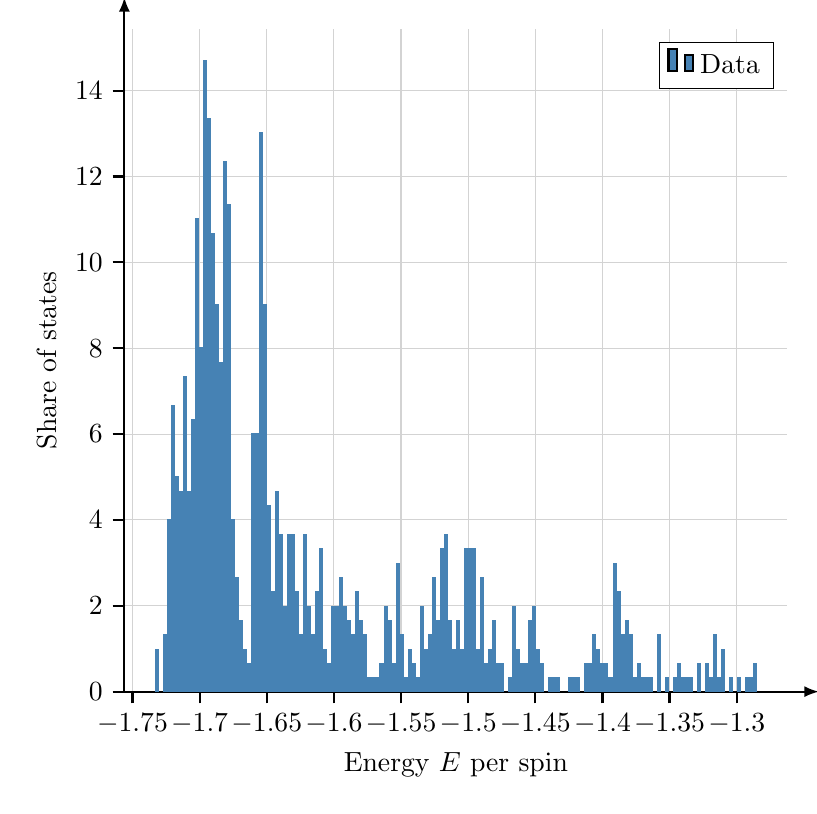
\begin{tikzpicture}

\definecolor{lightgray}{RGB}{211,211,211}
\definecolor{steelblue}{RGB}{70,130,180}

\begin{axis}[
tick align=outside,
tick pos=left,
x grid style={lightgray},
xlabel={Energy \(\displaystyle E\) per spin},
xmajorgrids,
xmin=-1.75604, xmax=-1.26236,
xtick style={color=black},
y grid style={lightgray},
ylabel={Share of states},
ymajorgrids,
ymin=0, ymax=15.4411764705877,
ytick style={color=black}
]
\draw[draw=none,fill=steelblue] (axis cs:-1.7336,0) rectangle (axis cs:-1.730608,1.00267379679141);
\addlegendimage{ybar,ybar legend,draw=none,fill=steelblue}
\addlegendentry{Data}

\draw[draw=none,fill=steelblue] (axis cs:-1.730608,0) rectangle (axis cs:-1.727616,0);
\draw[draw=none,fill=steelblue] (axis cs:-1.727616,0) rectangle (axis cs:-1.724624,1.33689839572188);
\draw[draw=none,fill=steelblue] (axis cs:-1.724624,0) rectangle (axis cs:-1.721632,4.01069518716593);
\draw[draw=none,fill=steelblue] (axis cs:-1.721632,0) rectangle (axis cs:-1.71864,6.68449197860939);
\draw[draw=none,fill=steelblue] (axis cs:-1.71864,0) rectangle (axis cs:-1.715648,5.01336898395741);
\draw[draw=none,fill=steelblue] (axis cs:-1.715648,0) rectangle (axis cs:-1.712656,4.67914438502657);
\draw[draw=none,fill=steelblue] (axis cs:-1.712656,0) rectangle (axis cs:-1.709664,7.35294117647087);
\draw[draw=none,fill=steelblue] (axis cs:-1.709664,0) rectangle (axis cs:-1.706672,4.67914438502657);
\draw[draw=none,fill=steelblue] (axis cs:-1.706672,0) rectangle (axis cs:-1.70368,6.35026737967939);
\draw[draw=none,fill=steelblue] (axis cs:-1.70368,0) rectangle (axis cs:-1.700688,11.0294117647055);
\draw[draw=none,fill=steelblue] (axis cs:-1.700688,0) rectangle (axis cs:-1.697696,8.02139037433186);
\draw[draw=none,fill=steelblue] (axis cs:-1.697696,0) rectangle (axis cs:-1.694704,14.7058823529407);
\draw[draw=none,fill=steelblue] (axis cs:-1.694704,0) rectangle (axis cs:-1.691712,13.3689839572198);
\draw[draw=none,fill=steelblue] (axis cs:-1.691712,0) rectangle (axis cs:-1.68872,10.695187165775);
\draw[draw=none,fill=steelblue] (axis cs:-1.68872,0) rectangle (axis cs:-1.685728,9.02406417112335);
\draw[draw=none,fill=steelblue] (axis cs:-1.685728,0) rectangle (axis cs:-1.682736,7.6871657754008);
\draw[draw=none,fill=steelblue] (axis cs:-1.682736,0) rectangle (axis cs:-1.679744,12.3663101604274);
\draw[draw=none,fill=steelblue] (axis cs:-1.679744,0) rectangle (axis cs:-1.676752,11.3636363636368);
\draw[draw=none,fill=steelblue] (axis cs:-1.676752,0) rectangle (axis cs:-1.67376,4.01069518716563);
\draw[draw=none,fill=steelblue] (axis cs:-1.67376,0) rectangle (axis cs:-1.670768,2.67379679144395);
\draw[draw=none,fill=steelblue] (axis cs:-1.670768,0) rectangle (axis cs:-1.667776,1.67112299465235);
\draw[draw=none,fill=steelblue] (axis cs:-1.667776,0) rectangle (axis cs:-1.664784,1.00267379679148);
\draw[draw=none,fill=steelblue] (axis cs:-1.664784,0) rectangle (axis cs:-1.661792,0.668449197860939);
\draw[draw=none,fill=steelblue] (axis cs:-1.661792,0) rectangle (axis cs:-1.6588,6.0160427807489);
\draw[draw=none,fill=steelblue] (axis cs:-1.6588,0) rectangle (axis cs:-1.655808,6.01604278074845);
\draw[draw=none,fill=steelblue] (axis cs:-1.655808,0) rectangle (axis cs:-1.652816,13.0347593582893);
\draw[draw=none,fill=steelblue] (axis cs:-1.652816,0) rectangle (axis cs:-1.649824,9.02406417112268);
\draw[draw=none,fill=steelblue] (axis cs:-1.649824,0) rectangle (axis cs:-1.646832,4.34491978609643);
\draw[draw=none,fill=steelblue] (axis cs:-1.646832,0) rectangle (axis cs:-1.64384,2.33957219251329);
\draw[draw=none,fill=steelblue] (axis cs:-1.64384,0) rectangle (axis cs:-1.640848,4.67914438502692);
\draw[draw=none,fill=steelblue] (axis cs:-1.640848,0) rectangle (axis cs:-1.637856,3.67647058823516);
\draw[draw=none,fill=steelblue] (axis cs:-1.637856,0) rectangle (axis cs:-1.634864,2.00534759358297);
\draw[draw=none,fill=steelblue] (axis cs:-1.634864,0) rectangle (axis cs:-1.631872,3.67647058823516);
\draw[draw=none,fill=steelblue] (axis cs:-1.631872,0) rectangle (axis cs:-1.62888,3.67647058823544);
\draw[draw=none,fill=steelblue] (axis cs:-1.62888,0) rectangle (axis cs:-1.625888,2.33957219251329);
\draw[draw=none,fill=steelblue] (axis cs:-1.625888,0) rectangle (axis cs:-1.622896,1.33689839572188);
\draw[draw=none,fill=steelblue] (axis cs:-1.622896,0) rectangle (axis cs:-1.619904,3.67647058823544);
\draw[draw=none,fill=steelblue] (axis cs:-1.619904,0) rectangle (axis cs:-1.616912,2.00534759358282);
\draw[draw=none,fill=steelblue] (axis cs:-1.616912,0) rectangle (axis cs:-1.61392,1.33689839572198);
\draw[draw=none,fill=steelblue] (axis cs:-1.61392,0) rectangle (axis cs:-1.610928,2.33957219251329);
\draw[draw=none,fill=steelblue] (axis cs:-1.610928,0) rectangle (axis cs:-1.607936,3.34224598930494);
\draw[draw=none,fill=steelblue] (axis cs:-1.607936,0) rectangle (axis cs:-1.604944,1.00267379679141);
\draw[draw=none,fill=steelblue] (axis cs:-1.604944,0) rectangle (axis cs:-1.601952,0.668449197860989);
\draw[draw=none,fill=steelblue] (axis cs:-1.601952,0) rectangle (axis cs:-1.59896,2.00534759358282);
\draw[draw=none,fill=steelblue] (axis cs:-1.59896,0) rectangle (axis cs:-1.595968,2.00534759358297);
\draw[draw=none,fill=steelblue] (axis cs:-1.595968,0) rectangle (axis cs:-1.592976,2.67379679144376);
\draw[draw=none,fill=steelblue] (axis cs:-1.592976,0) rectangle (axis cs:-1.589984,2.00534759358297);
\draw[draw=none,fill=steelblue] (axis cs:-1.589984,0) rectangle (axis cs:-1.586992,1.67112299465235);
\draw[draw=none,fill=steelblue] (axis cs:-1.586992,0) rectangle (axis cs:-1.584,1.33689839572198);
\draw[draw=none,fill=steelblue] (axis cs:-1.584,0) rectangle (axis cs:-1.581008,2.33957219251329);
\draw[draw=none,fill=steelblue] (axis cs:-1.581008,0) rectangle (axis cs:-1.578016,1.67112299465247);
\draw[draw=none,fill=steelblue] (axis cs:-1.578016,0) rectangle (axis cs:-1.575024,1.33689839572188);
\draw[draw=none,fill=steelblue] (axis cs:-1.575024,0) rectangle (axis cs:-1.572032,0.334224598930494);
\draw[draw=none,fill=steelblue] (axis cs:-1.572032,0) rectangle (axis cs:-1.56904,0.334224598930469);
\draw[draw=none,fill=steelblue] (axis cs:-1.56904,0) rectangle (axis cs:-1.566048,0.334224598930469);
\draw[draw=none,fill=steelblue] (axis cs:-1.566048,0) rectangle (axis cs:-1.563056,0.668449197860989);
\draw[draw=none,fill=steelblue] (axis cs:-1.563056,0) rectangle (axis cs:-1.560064,2.00534759358282);
\draw[draw=none,fill=steelblue] (axis cs:-1.560064,0) rectangle (axis cs:-1.557072,1.67112299465247);
\draw[draw=none,fill=steelblue] (axis cs:-1.557072,0) rectangle (axis cs:-1.55408,0.668449197860939);
\draw[draw=none,fill=steelblue] (axis cs:-1.55408,0) rectangle (axis cs:-1.551088,3.00802139037445);
\draw[draw=none,fill=steelblue] (axis cs:-1.551088,0) rectangle (axis cs:-1.548096,1.33689839572188);
\draw[draw=none,fill=steelblue] (axis cs:-1.548096,0) rectangle (axis cs:-1.545104,0.334224598930494);
\draw[draw=none,fill=steelblue] (axis cs:-1.545104,0) rectangle (axis cs:-1.542112,1.00267379679141);
\draw[draw=none,fill=steelblue] (axis cs:-1.542112,0) rectangle (axis cs:-1.53912,0.668449197860989);
\draw[draw=none,fill=steelblue] (axis cs:-1.53912,0) rectangle (axis cs:-1.536128,0.334224598930469);
\draw[draw=none,fill=steelblue] (axis cs:-1.536128,0) rectangle (axis cs:-1.533136,2.00534759358297);
\draw[draw=none,fill=steelblue] (axis cs:-1.533136,0) rectangle (axis cs:-1.530144,1.00267379679141);
\draw[draw=none,fill=steelblue] (axis cs:-1.530144,0) rectangle (axis cs:-1.527152,1.33689839572198);
\draw[draw=none,fill=steelblue] (axis cs:-1.527152,0) rectangle (axis cs:-1.52416,2.67379679144376);
\draw[draw=none,fill=steelblue] (axis cs:-1.52416,0) rectangle (axis cs:-1.521168,1.67112299465235);
\draw[draw=none,fill=steelblue] (axis cs:-1.521168,0) rectangle (axis cs:-1.518176,3.34224598930494);
\draw[draw=none,fill=steelblue] (axis cs:-1.518176,0) rectangle (axis cs:-1.515184,3.67647058823544);
\draw[draw=none,fill=steelblue] (axis cs:-1.515184,0) rectangle (axis cs:-1.512192,1.67112299465235);
\draw[draw=none,fill=steelblue] (axis cs:-1.512192,0) rectangle (axis cs:-1.5092,1.00267379679141);
\draw[draw=none,fill=steelblue] (axis cs:-1.5092,0) rectangle (axis cs:-1.506208,1.67112299465247);
\draw[draw=none,fill=steelblue] (axis cs:-1.506208,0) rectangle (axis cs:-1.503216,1.00267379679141);
\draw[draw=none,fill=steelblue] (axis cs:-1.503216,0) rectangle (axis cs:-1.500224,3.34224598930494);
\draw[draw=none,fill=steelblue] (axis cs:-1.500224,0) rectangle (axis cs:-1.497232,3.34224598930469);
\draw[draw=none,fill=steelblue] (axis cs:-1.497232,0) rectangle (axis cs:-1.49424,3.34224598930494);
\draw[draw=none,fill=steelblue] (axis cs:-1.49424,0) rectangle (axis cs:-1.491248,1.00267379679141);
\draw[draw=none,fill=steelblue] (axis cs:-1.491248,0) rectangle (axis cs:-1.488256,2.67379679144395);
\draw[draw=none,fill=steelblue] (axis cs:-1.488256,0) rectangle (axis cs:-1.485264,0.668449197860939);
\draw[draw=none,fill=steelblue] (axis cs:-1.485264,0) rectangle (axis cs:-1.482272,1.00267379679148);
\draw[draw=none,fill=steelblue] (axis cs:-1.482272,0) rectangle (axis cs:-1.47928,1.67112299465235);
\draw[draw=none,fill=steelblue] (axis cs:-1.47928,0) rectangle (axis cs:-1.476288,0.668449197860989);
\draw[draw=none,fill=steelblue] (axis cs:-1.476288,0) rectangle (axis cs:-1.473296,0.668449197860939);
\draw[draw=none,fill=steelblue] (axis cs:-1.473296,0) rectangle (axis cs:-1.470304,0);
\draw[draw=none,fill=steelblue] (axis cs:-1.470304,0) rectangle (axis cs:-1.467312,0.334224598930469);
\draw[draw=none,fill=steelblue] (axis cs:-1.467312,0) rectangle (axis cs:-1.46432,2.00534759358282);
\draw[draw=none,fill=steelblue] (axis cs:-1.46432,0) rectangle (axis cs:-1.461328,1.00267379679148);
\draw[draw=none,fill=steelblue] (axis cs:-1.461328,0) rectangle (axis cs:-1.458336,0.668449197860989);
\draw[draw=none,fill=steelblue] (axis cs:-1.458336,0) rectangle (axis cs:-1.455344,0.668449197860939);
\draw[draw=none,fill=steelblue] (axis cs:-1.455344,0) rectangle (axis cs:-1.452352,1.67112299465235);
\draw[draw=none,fill=steelblue] (axis cs:-1.452352,0) rectangle (axis cs:-1.44936,2.00534759358297);
\draw[draw=none,fill=steelblue] (axis cs:-1.44936,0) rectangle (axis cs:-1.446368,1.00267379679148);
\draw[draw=none,fill=steelblue] (axis cs:-1.446368,0) rectangle (axis cs:-1.443376,0.668449197860939);
\draw[draw=none,fill=steelblue] (axis cs:-1.443376,0) rectangle (axis cs:-1.440384,0);
\draw[draw=none,fill=steelblue] (axis cs:-1.440384,0) rectangle (axis cs:-1.437392,0.334224598930494);
\draw[draw=none,fill=steelblue] (axis cs:-1.437392,0) rectangle (axis cs:-1.4344,0.334224598930469);
\draw[draw=none,fill=steelblue] (axis cs:-1.4344,0) rectangle (axis cs:-1.431408,0.334224598930494);
\draw[draw=none,fill=steelblue] (axis cs:-1.431408,0) rectangle (axis cs:-1.428416,0);
\draw[draw=none,fill=steelblue] (axis cs:-1.428416,0) rectangle (axis cs:-1.425424,0);
\draw[draw=none,fill=steelblue] (axis cs:-1.425424,0) rectangle (axis cs:-1.422432,0.334224598930469);
\draw[draw=none,fill=steelblue] (axis cs:-1.422432,0) rectangle (axis cs:-1.41944,0.334224598930494);
\draw[draw=none,fill=steelblue] (axis cs:-1.41944,0) rectangle (axis cs:-1.416448,0.334224598930469);
\draw[draw=none,fill=steelblue] (axis cs:-1.416448,0) rectangle (axis cs:-1.413456,0);
\draw[draw=none,fill=steelblue] (axis cs:-1.413456,0) rectangle (axis cs:-1.410464,0.668449197860939);
\draw[draw=none,fill=steelblue] (axis cs:-1.410464,0) rectangle (axis cs:-1.407472,0.668449197860939);
\draw[draw=none,fill=steelblue] (axis cs:-1.407472,0) rectangle (axis cs:-1.40448,1.33689839572198);
\draw[draw=none,fill=steelblue] (axis cs:-1.40448,0) rectangle (axis cs:-1.401488,1.00267379679148);
\draw[draw=none,fill=steelblue] (axis cs:-1.401488,0) rectangle (axis cs:-1.398496,0.668449197860939);
\draw[draw=none,fill=steelblue] (axis cs:-1.398496,0) rectangle (axis cs:-1.395504,0.668449197860939);
\draw[draw=none,fill=steelblue] (axis cs:-1.395504,0) rectangle (axis cs:-1.392512,0.334224598930494);
\draw[draw=none,fill=steelblue] (axis cs:-1.392512,0) rectangle (axis cs:-1.38952,3.00802139037423);
\draw[draw=none,fill=steelblue] (axis cs:-1.38952,0) rectangle (axis cs:-1.386528,2.33957219251346);
\draw[draw=none,fill=steelblue] (axis cs:-1.386528,0) rectangle (axis cs:-1.383536,1.33689839572188);
\draw[draw=none,fill=steelblue] (axis cs:-1.383536,0) rectangle (axis cs:-1.380544,1.67112299465247);
\draw[draw=none,fill=steelblue] (axis cs:-1.380544,0) rectangle (axis cs:-1.377552,1.33689839572188);
\draw[draw=none,fill=steelblue] (axis cs:-1.377552,0) rectangle (axis cs:-1.37456,0.334224598930494);
\draw[draw=none,fill=steelblue] (axis cs:-1.37456,0) rectangle (axis cs:-1.371568,0.668449197860939);
\draw[draw=none,fill=steelblue] (axis cs:-1.371568,0) rectangle (axis cs:-1.368576,0.334224598930494);
\draw[draw=none,fill=steelblue] (axis cs:-1.368576,0) rectangle (axis cs:-1.365584,0.334224598930469);
\draw[draw=none,fill=steelblue] (axis cs:-1.365584,0) rectangle (axis cs:-1.362592,0.334224598930469);
\draw[draw=none,fill=steelblue] (axis cs:-1.362592,0) rectangle (axis cs:-1.3596,0);
\draw[draw=none,fill=steelblue] (axis cs:-1.3596,0) rectangle (axis cs:-1.356608,1.33689839572198);
\draw[draw=none,fill=steelblue] (axis cs:-1.356608,0) rectangle (axis cs:-1.353616,0);
\draw[draw=none,fill=steelblue] (axis cs:-1.353616,0) rectangle (axis cs:-1.350624,0.334224598930469);
\draw[draw=none,fill=steelblue] (axis cs:-1.350624,0) rectangle (axis cs:-1.347632,0);
\draw[draw=none,fill=steelblue] (axis cs:-1.347632,0) rectangle (axis cs:-1.34464,0.334224598930494);
\draw[draw=none,fill=steelblue] (axis cs:-1.34464,0) rectangle (axis cs:-1.341648,0.668449197860939);
\draw[draw=none,fill=steelblue] (axis cs:-1.341648,0) rectangle (axis cs:-1.338656,0.334224598930469);
\draw[draw=none,fill=steelblue] (axis cs:-1.338656,0) rectangle (axis cs:-1.335664,0.334224598930494);
\draw[draw=none,fill=steelblue] (axis cs:-1.335664,0) rectangle (axis cs:-1.332672,0.334224598930469);
\draw[draw=none,fill=steelblue] (axis cs:-1.332672,0) rectangle (axis cs:-1.32968,0);
\draw[draw=none,fill=steelblue] (axis cs:-1.32968,0) rectangle (axis cs:-1.326688,0.668449197860939);
\draw[draw=none,fill=steelblue] (axis cs:-1.326688,0) rectangle (axis cs:-1.323696,0);
\draw[draw=none,fill=steelblue] (axis cs:-1.323696,0) rectangle (axis cs:-1.320704,0.668449197860939);
\draw[draw=none,fill=steelblue] (axis cs:-1.320704,0) rectangle (axis cs:-1.317712,0.334224598930494);
\draw[draw=none,fill=steelblue] (axis cs:-1.317712,0) rectangle (axis cs:-1.31472,1.33689839572188);
\draw[draw=none,fill=steelblue] (axis cs:-1.31472,0) rectangle (axis cs:-1.311728,0.334224598930494);
\draw[draw=none,fill=steelblue] (axis cs:-1.311728,0) rectangle (axis cs:-1.308736,1.00267379679141);
\draw[draw=none,fill=steelblue] (axis cs:-1.308736,0) rectangle (axis cs:-1.305744,0);
\draw[draw=none,fill=steelblue] (axis cs:-1.305744,0) rectangle (axis cs:-1.302752,0.334224598930494);
\draw[draw=none,fill=steelblue] (axis cs:-1.302752,0) rectangle (axis cs:-1.29976,0);
\draw[draw=none,fill=steelblue] (axis cs:-1.29976,0) rectangle (axis cs:-1.296768,0.334224598930469);
\draw[draw=none,fill=steelblue] (axis cs:-1.296768,0) rectangle (axis cs:-1.293776,0);
\draw[draw=none,fill=steelblue] (axis cs:-1.293776,0) rectangle (axis cs:-1.290784,0.334224598930494);
\draw[draw=none,fill=steelblue] (axis cs:-1.290784,0) rectangle (axis cs:-1.287792,0.334224598930494);
\draw[draw=none,fill=steelblue] (axis cs:-1.287792,0) rectangle (axis cs:-1.2848,0.668449197860939);
\end{axis}

\end{tikzpicture}

\end{figure}

\begin{figure}
\centering
% This file was created with tikzplotlib v0.10.1.
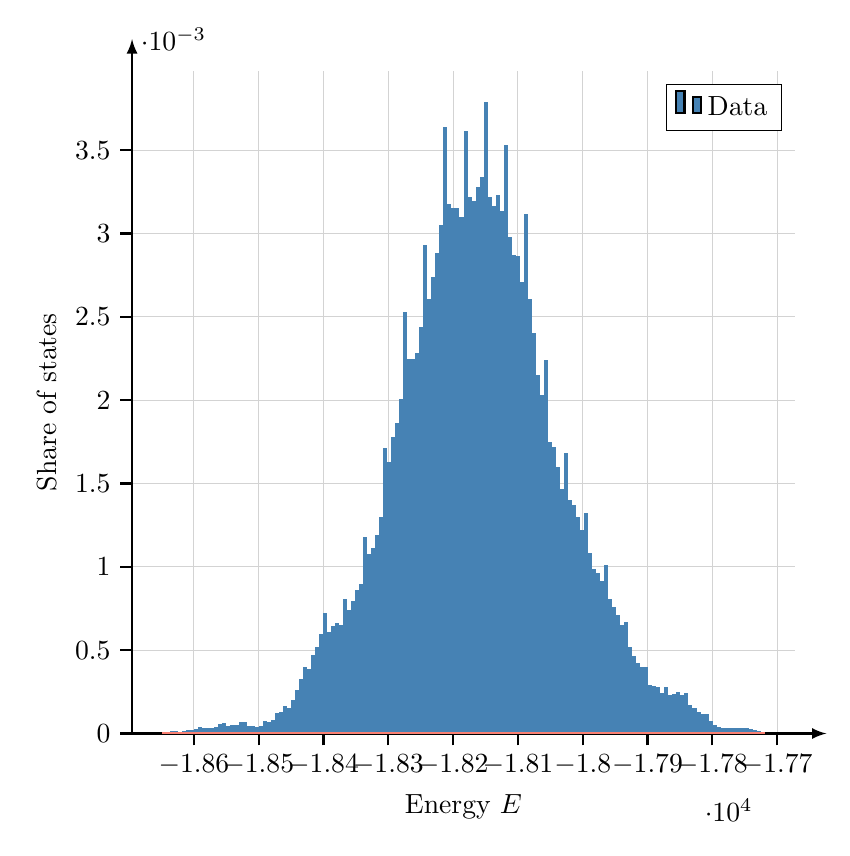
\begin{tikzpicture}

\definecolor{lightgray}{RGB}{211,211,211}
\definecolor{salmon}{RGB}{250,128,114}
\definecolor{steelblue}{RGB}{70,130,180}

\begin{axis}[
tick align=outside,
tick pos=left,
x grid style={lightgray},
xlabel={Energy \(\displaystyle E\)},
xmajorgrids,
xmin=-18695.5, xmax=-17672.5,
xtick style={color=black},
y grid style={lightgray},
ylabel={Share of states},
ymajorgrids,
ymin=0, ymax=0.00397727016128986,
ytick style={color=black}
]
\draw[draw=none,fill=steelblue] (axis cs:-18649,0) rectangle (axis cs:-18642.8,2.7822580645158e-06);
\addlegendimage{ybar,ybar legend,draw=none,fill=steelblue}
\addlegendentry{Data}

\draw[draw=none,fill=steelblue] (axis cs:-18642.8,0) rectangle (axis cs:-18636.6,6.97580645161208e-06);
\draw[draw=none,fill=steelblue] (axis cs:-18636.6,0) rectangle (axis cs:-18630.4,1.23790322580703e-05);
\draw[draw=none,fill=steelblue] (axis cs:-18630.4,0) rectangle (axis cs:-18624.2,1.60887096774175e-05);
\draw[draw=none,fill=steelblue] (axis cs:-18624.2,0) rectangle (axis cs:-18618,9.74462365591284e-06);
\draw[draw=none,fill=steelblue] (axis cs:-18618,0) rectangle (axis cs:-18611.8,1.58064516129014e-05);
\draw[draw=none,fill=steelblue] (axis cs:-18611.8,0) rectangle (axis cs:-18605.6,1.81451612903205e-05);
\draw[draw=none,fill=steelblue] (axis cs:-18605.6,0) rectangle (axis cs:-18599.4,2.34005376344196e-05);
\draw[draw=none,fill=steelblue] (axis cs:-18599.4,0) rectangle (axis cs:-18593.2,2.78629032258032e-05);
\draw[draw=none,fill=steelblue] (axis cs:-18593.2,0) rectangle (axis cs:-18587,3.70161290322537e-05);
\draw[draw=none,fill=steelblue] (axis cs:-18587,0) rectangle (axis cs:-18580.8,3.27688172042972e-05);
\draw[draw=none,fill=steelblue] (axis cs:-18580.8,0) rectangle (axis cs:-18574.6,3.30913978494585e-05);
\draw[draw=none,fill=steelblue] (axis cs:-18574.6,0) rectangle (axis cs:-18568.4,3.6021505376361e-05);
\draw[draw=none,fill=steelblue] (axis cs:-18568.4,0) rectangle (axis cs:-18562.2,3.90188172042965e-05);
\draw[draw=none,fill=steelblue] (axis cs:-18562.2,0) rectangle (axis cs:-18556,5.63844086021439e-05);
\draw[draw=none,fill=steelblue] (axis cs:-18556,0) rectangle (axis cs:-18549.8,6.13306451612831e-05);
\draw[draw=none,fill=steelblue] (axis cs:-18549.8,0) rectangle (axis cs:-18543.6,4.65725806451558e-05);
\draw[draw=none,fill=steelblue] (axis cs:-18543.6,0) rectangle (axis cs:-18537.4,5.20833333333578e-05);
\draw[draw=none,fill=steelblue] (axis cs:-18537.4,0) rectangle (axis cs:-18531.2,5.20564516128971e-05);
\draw[draw=none,fill=steelblue] (axis cs:-18531.2,0) rectangle (axis cs:-18525,6.67741935483793e-05);
\draw[draw=none,fill=steelblue] (axis cs:-18525,0) rectangle (axis cs:-18518.8,6.90725806451532e-05);
\draw[draw=none,fill=steelblue] (axis cs:-18518.8,0) rectangle (axis cs:-18512.6,4.71908602150482e-05);
\draw[draw=none,fill=steelblue] (axis cs:-18512.6,0) rectangle (axis cs:-18506.4,4.21639784946434e-05);
\draw[draw=none,fill=steelblue] (axis cs:-18506.4,0) rectangle (axis cs:-18500.2,3.74059139784902e-05);
\draw[draw=none,fill=steelblue] (axis cs:-18500.2,0) rectangle (axis cs:-18494,4.57526881720376e-05);
\draw[draw=none,fill=steelblue] (axis cs:-18494,0) rectangle (axis cs:-18487.8,7.56586021505288e-05);
\draw[draw=none,fill=steelblue] (axis cs:-18487.8,0) rectangle (axis cs:-18481.6,6.75403225806372e-05);
\draw[draw=none,fill=steelblue] (axis cs:-18481.6,0) rectangle (axis cs:-18475.4,8.13306451613285e-05);
\draw[draw=none,fill=steelblue] (axis cs:-18475.4,0) rectangle (axis cs:-18469.2,0.000121962365591384);
\draw[draw=none,fill=steelblue] (axis cs:-18469.2,0) rectangle (axis cs:-18463,0.000126922043010738);
\draw[draw=none,fill=steelblue] (axis cs:-18463,0) rectangle (axis cs:-18456.8,0.000163911290322561);
\draw[draw=none,fill=steelblue] (axis cs:-18456.8,0) rectangle (axis cs:-18450.6,0.000155053763440842);
\draw[draw=none,fill=steelblue] (axis cs:-18450.6,0) rectangle (axis cs:-18444.4,0.000198346774193641);
\draw[draw=none,fill=steelblue] (axis cs:-18444.4,0) rectangle (axis cs:-18438.2,0.000261290322580615);
\draw[draw=none,fill=steelblue] (axis cs:-18438.2,0) rectangle (axis cs:-18432,0.00032451612903222);
\draw[draw=none,fill=steelblue] (axis cs:-18432,0) rectangle (axis cs:-18425.8,0.000401935483870921);
\draw[draw=none,fill=steelblue] (axis cs:-18425.8,0) rectangle (axis cs:-18419.6,0.000387325268817159);
\draw[draw=none,fill=steelblue] (axis cs:-18419.6,0) rectangle (axis cs:-18413.4,0.000471357526881942);
\draw[draw=none,fill=steelblue] (axis cs:-18413.4,0) rectangle (axis cs:-18407.2,0.000520403225806391);
\draw[draw=none,fill=steelblue] (axis cs:-18407.2,0) rectangle (axis cs:-18401,0.000597782258064446);
\draw[draw=none,fill=steelblue] (axis cs:-18401,0) rectangle (axis cs:-18394.8,0.000724811827956904);
\draw[draw=none,fill=steelblue] (axis cs:-18394.8,0) rectangle (axis cs:-18388.6,0.00060779569892466);
\draw[draw=none,fill=steelblue] (axis cs:-18388.6,0) rectangle (axis cs:-18382.4,0.000643225806451915);
\draw[draw=none,fill=steelblue] (axis cs:-18382.4,0) rectangle (axis cs:-18376.2,0.00066193548387089);
\draw[draw=none,fill=steelblue] (axis cs:-18376.2,0) rectangle (axis cs:-18370,0.000653198924731106);
\draw[draw=none,fill=steelblue] (axis cs:-18370,0) rectangle (axis cs:-18363.8,0.000807580645161196);
\draw[draw=none,fill=steelblue] (axis cs:-18363.8,0) rectangle (axis cs:-18357.6,0.000739731182795612);
\draw[draw=none,fill=steelblue] (axis cs:-18357.6,0) rectangle (axis cs:-18351.4,0.000794704301075642);
\draw[draw=none,fill=steelblue] (axis cs:-18351.4,0) rectangle (axis cs:-18345.2,0.000862970430107426);
\draw[draw=none,fill=steelblue] (axis cs:-18345.2,0) rectangle (axis cs:-18339,0.000897997311827852);
\draw[draw=none,fill=steelblue] (axis cs:-18339,0) rectangle (axis cs:-18332.8,0.00117622311827943);
\draw[draw=none,fill=steelblue] (axis cs:-18332.8,0) rectangle (axis cs:-18326.6,0.00107508064516116);
\draw[draw=none,fill=steelblue] (axis cs:-18326.6,0) rectangle (axis cs:-18320.4,0.00111463709677472);
\draw[draw=none,fill=steelblue] (axis cs:-18320.4,0) rectangle (axis cs:-18314.2,0.00119270161290309);
\draw[draw=none,fill=steelblue] (axis cs:-18314.2,0) rectangle (axis cs:-18308,0.00129787634408587);
\draw[draw=none,fill=steelblue] (axis cs:-18308,0) rectangle (axis cs:-18301.8,0.00171325268817184);
\draw[draw=none,fill=steelblue] (axis cs:-18301.8,0) rectangle (axis cs:-18295.6,0.00162965053763422);
\draw[draw=none,fill=steelblue] (axis cs:-18295.6,0) rectangle (axis cs:-18289.4,0.00177830645161374);
\draw[draw=none,fill=steelblue] (axis cs:-18289.4,0) rectangle (axis cs:-18283.2,0.00186279569892451);
\draw[draw=none,fill=steelblue] (axis cs:-18283.2,0) rectangle (axis cs:-18277,0.00200639784946213);
\draw[draw=none,fill=steelblue] (axis cs:-18277,0) rectangle (axis cs:-18270.8,0.00252631720430078);
\draw[draw=none,fill=steelblue] (axis cs:-18270.8,0) rectangle (axis cs:-18264.6,0.00224495967741909);
\draw[draw=none,fill=steelblue] (axis cs:-18264.6,0) rectangle (axis cs:-18258.4,0.00224881720430213);
\draw[draw=none,fill=steelblue] (axis cs:-18258.4,0) rectangle (axis cs:-18252.2,0.002284704301075);
\draw[draw=none,fill=steelblue] (axis cs:-18252.2,0) rectangle (axis cs:-18246,0.00243744623655885);
\draw[draw=none,fill=steelblue] (axis cs:-18246,0) rectangle (axis cs:-18239.8,0.00293357526881686);
\draw[draw=none,fill=steelblue] (axis cs:-18239.8,0) rectangle (axis cs:-18233.6,0.00260822580645131);
\draw[draw=none,fill=steelblue] (axis cs:-18233.6,0) rectangle (axis cs:-18227.4,0.00273629032258193);
\draw[draw=none,fill=steelblue] (axis cs:-18227.4,0) rectangle (axis cs:-18221.2,0.00288336021505342);
\draw[draw=none,fill=steelblue] (axis cs:-18221.2,0) rectangle (axis cs:-18215,0.00304819892473083);
\draw[draw=none,fill=steelblue] (axis cs:-18215,0) rectangle (axis cs:-18208.8,0.00364107526881678);
\draw[draw=none,fill=steelblue] (axis cs:-18208.8,0) rectangle (axis cs:-18202.6,0.00317740591397812);
\draw[draw=none,fill=steelblue] (axis cs:-18202.6,0) rectangle (axis cs:-18196.4,0.00315211021505524);
\draw[draw=none,fill=steelblue] (axis cs:-18196.4,0) rectangle (axis cs:-18190.2,0.00315352150537597);
\draw[draw=none,fill=steelblue] (axis cs:-18190.2,0) rectangle (axis cs:-18184,0.00309724462365555);
\draw[draw=none,fill=steelblue] (axis cs:-18184,0) rectangle (axis cs:-18177.8,0.00361771505376302);
\draw[draw=none,fill=steelblue] (axis cs:-18177.8,0) rectangle (axis cs:-18171.6,0.00321954301075231);
\draw[draw=none,fill=steelblue] (axis cs:-18171.6,0) rectangle (axis cs:-18165.4,0.00319783602150688);
\draw[draw=none,fill=steelblue] (axis cs:-18165.4,0) rectangle (axis cs:-18159.2,0.0032814112903222);
\draw[draw=none,fill=steelblue] (axis cs:-18159.2,0) rectangle (axis cs:-18153,0.00334104838709638);
\draw[draw=none,fill=steelblue] (axis cs:-18153,0) rectangle (axis cs:-18146.8,0.00378787634408558);
\draw[draw=none,fill=steelblue] (axis cs:-18146.8,0) rectangle (axis cs:-18140.6,0.00322056451612865);
\draw[draw=none,fill=steelblue] (axis cs:-18140.6,0) rectangle (axis cs:-18134.4,0.00316668010752837);
\draw[draw=none,fill=steelblue] (axis cs:-18134.4,0) rectangle (axis cs:-18128.2,0.00323397849462328);
\draw[draw=none,fill=steelblue] (axis cs:-18128.2,0) rectangle (axis cs:-18122,0.00313802419354802);
\draw[draw=none,fill=steelblue] (axis cs:-18122,0) rectangle (axis cs:-18115.8,0.00353314516128991);
\draw[draw=none,fill=steelblue] (axis cs:-18115.8,0) rectangle (axis cs:-18109.6,0.00298122311827922);
\draw[draw=none,fill=steelblue] (axis cs:-18109.6,0) rectangle (axis cs:-18103.4,0.00287158602150672);
\draw[draw=none,fill=steelblue] (axis cs:-18103.4,0) rectangle (axis cs:-18097.2,0.00286290322580612);
\draw[draw=none,fill=steelblue] (axis cs:-18097.2,0) rectangle (axis cs:-18091,0.00271009408602119);
\draw[draw=none,fill=steelblue] (axis cs:-18091,0) rectangle (axis cs:-18084.8,0.00311413978494587);
\draw[draw=none,fill=steelblue] (axis cs:-18084.8,0) rectangle (axis cs:-18078.6,0.00260903225806421);
\draw[draw=none,fill=steelblue] (axis cs:-18078.6,0) rectangle (axis cs:-18072.4,0.00240049731182908);
\draw[draw=none,fill=steelblue] (axis cs:-18072.4,0) rectangle (axis cs:-18066.2,0.00214814516129007);
\draw[draw=none,fill=steelblue] (axis cs:-18066.2,0) rectangle (axis cs:-18060,0.00203080645161266);
\draw[draw=none,fill=steelblue] (axis cs:-18060,0) rectangle (axis cs:-18053.8,0.00224401881720404);
\draw[draw=none,fill=steelblue] (axis cs:-18053.8,0) rectangle (axis cs:-18047.6,0.00174838709677399);
\draw[draw=none,fill=steelblue] (axis cs:-18047.6,0) rectangle (axis cs:-18041.4,0.00171670698924812);
\draw[draw=none,fill=steelblue] (axis cs:-18041.4,0) rectangle (axis cs:-18035.2,0.00160076612903207);
\draw[draw=none,fill=steelblue] (axis cs:-18035.2,0) rectangle (axis cs:-18029,0.00146435483870951);
\draw[draw=none,fill=steelblue] (axis cs:-18029,0) rectangle (axis cs:-18022.8,0.00168530913978475);
\draw[draw=none,fill=steelblue] (axis cs:-18022.8,0) rectangle (axis cs:-18016.6,0.00140114247311811);
\draw[draw=none,fill=steelblue] (axis cs:-18016.6,0) rectangle (axis cs:-18010.4,0.00137293010752753);
\draw[draw=none,fill=steelblue] (axis cs:-18010.4,0) rectangle (axis cs:-18004.2,0.0012986155913977);
\draw[draw=none,fill=steelblue] (axis cs:-18004.2,0) rectangle (axis cs:-17998,0.001218696236559);
\draw[draw=none,fill=steelblue] (axis cs:-17998,0) rectangle (axis cs:-17991.8,0.00132434139784931);
\draw[draw=none,fill=steelblue] (axis cs:-17991.8,0) rectangle (axis cs:-17985.6,0.00108364247311815);
\draw[draw=none,fill=steelblue] (axis cs:-17985.6,0) rectangle (axis cs:-17979.4,0.00099004032258111);
\draw[draw=none,fill=steelblue] (axis cs:-17979.4,0) rectangle (axis cs:-17973.2,0.000964395161290209);
\draw[draw=none,fill=steelblue] (axis cs:-17973.2,0) rectangle (axis cs:-17967,0.000915241935483764);
\draw[draw=none,fill=steelblue] (axis cs:-17967,0) rectangle (axis cs:-17960.8,0.00100948924731171);
\draw[draw=none,fill=steelblue] (axis cs:-17960.8,0) rectangle (axis cs:-17954.6,0.000808776881720335);
\draw[draw=none,fill=steelblue] (axis cs:-17954.6,0) rectangle (axis cs:-17948.4,0.000761827956989605);
\draw[draw=none,fill=steelblue] (axis cs:-17948.4,0) rectangle (axis cs:-17942.2,0.000711209677419271);
\draw[draw=none,fill=steelblue] (axis cs:-17942.2,0) rectangle (axis cs:-17936,0.000653817204300999);
\draw[draw=none,fill=steelblue] (axis cs:-17936,0) rectangle (axis cs:-17929.8,0.000666384408602072);
\draw[draw=none,fill=steelblue] (axis cs:-17929.8,0) rectangle (axis cs:-17923.6,0.000517002688171982);
\draw[draw=none,fill=steelblue] (axis cs:-17923.6,0) rectangle (axis cs:-17917.4,0.000467163978494843);
\draw[draw=none,fill=steelblue] (axis cs:-17917.4,0) rectangle (axis cs:-17911.2,0.000420282258064467);
\draw[draw=none,fill=steelblue] (axis cs:-17911.2,0) rectangle (axis cs:-17905,0.000400268817204254);
\draw[draw=none,fill=steelblue] (axis cs:-17905,0) rectangle (axis cs:-17898.8,0.000397473118279523);
\draw[draw=none,fill=steelblue] (axis cs:-17898.8,0) rectangle (axis cs:-17892.6,0.000290900537634374);
\draw[draw=none,fill=steelblue] (axis cs:-17892.6,0) rectangle (axis cs:-17886.4,0.00028751344086035);
\draw[draw=none,fill=steelblue] (axis cs:-17886.4,0) rectangle (axis cs:-17880.2,0.00027811827956986);
\draw[draw=none,fill=steelblue] (axis cs:-17880.2,0) rectangle (axis cs:-17874,0.000242755376344058);
\draw[draw=none,fill=steelblue] (axis cs:-17874,0) rectangle (axis cs:-17867.8,0.000276545698924699);
\draw[draw=none,fill=steelblue] (axis cs:-17867.8,0) rectangle (axis cs:-17861.6,0.000233010752688145);
\draw[draw=none,fill=steelblue] (axis cs:-17861.6,0) rectangle (axis cs:-17855.4,0.000238427419354951);
\draw[draw=none,fill=steelblue] (axis cs:-17855.4,0) rectangle (axis cs:-17849.2,0.000249368279569863);
\draw[draw=none,fill=steelblue] (axis cs:-17849.2,0) rectangle (axis cs:-17843,0.000230591397849435);
\draw[draw=none,fill=steelblue] (axis cs:-17843,0) rectangle (axis cs:-17836.8,0.00024456989247309);
\draw[draw=none,fill=steelblue] (axis cs:-17836.8,0) rectangle (axis cs:-17830.6,0.000170497311827937);
\draw[draw=none,fill=steelblue] (axis cs:-17830.6,0) rectangle (axis cs:-17824.4,0.000151599462365663);
\draw[draw=none,fill=steelblue] (axis cs:-17824.4,0) rectangle (axis cs:-17818.2,0.000130443548387081);
\draw[draw=none,fill=steelblue] (axis cs:-17818.2,0) rectangle (axis cs:-17812,0.00011979838709676);
\draw[draw=none,fill=steelblue] (axis cs:-17812,0) rectangle (axis cs:-17805.8,0.000116397849462352);
\draw[draw=none,fill=steelblue] (axis cs:-17805.8,0) rectangle (axis cs:-17799.6,7.43548387096687e-05);
\draw[draw=none,fill=steelblue] (axis cs:-17799.6,0) rectangle (axis cs:-17793.4,5.30779569892722e-05);
\draw[draw=none,fill=steelblue] (axis cs:-17793.4,0) rectangle (axis cs:-17787.2,3.95698924731136e-05);
\draw[draw=none,fill=steelblue] (axis cs:-17787.2,0) rectangle (axis cs:-17781,3.47311827956949e-05);
\draw[draw=none,fill=steelblue] (axis cs:-17781,0) rectangle (axis cs:-17774.8,3.23655913978457e-05);
\draw[draw=none,fill=steelblue] (axis cs:-17774.8,0) rectangle (axis cs:-17768.6,3.13172043010716e-05);
\draw[draw=none,fill=steelblue] (axis cs:-17768.6,0) rectangle (axis cs:-17762.4,3.55241935484038e-05);
\draw[draw=none,fill=steelblue] (axis cs:-17762.4,0) rectangle (axis cs:-17756.2,3.40725806451573e-05);
\draw[draw=none,fill=steelblue] (axis cs:-17756.2,0) rectangle (axis cs:-17750,3.01612903225771e-05);
\draw[draw=none,fill=steelblue] (axis cs:-17750,0) rectangle (axis cs:-17743.8,3.1424731182792e-05);
\draw[draw=none,fill=steelblue] (axis cs:-17743.8,0) rectangle (axis cs:-17737.6,2.63172043010722e-05);
\draw[draw=none,fill=steelblue] (axis cs:-17737.6,0) rectangle (axis cs:-17731.4,2.26747311828063e-05);
\draw[draw=none,fill=steelblue] (axis cs:-17731.4,0) rectangle (axis cs:-17725.2,1.42069892473102e-05);
\draw[draw=none,fill=steelblue] (axis cs:-17725.2,0) rectangle (axis cs:-17719,4.09946236559092e-06);
\addplot [salmon]
table {%
-18649 0
-18648.0690690691 0
-18647.1381381381 0
-18646.2072072072 0
-18645.2762762763 0
-18644.3453453453 0
-18643.4144144144 0
-18642.4834834835 0
-18641.5525525526 0
-18640.6216216216 0
-18639.6906906907 0
-18638.7597597598 0
-18637.8288288288 0
-18636.8978978979 0
-18635.966966967 0
-18635.036036036 0
-18634.1051051051 0
-18633.1741741742 0
-18632.2432432432 0
-18631.3123123123 0
-18630.3813813814 0
-18629.4504504505 0
-18628.5195195195 0
-18627.5885885886 0
-18626.6576576577 0
-18625.7267267267 0
-18624.7957957958 0
-18623.8648648649 0
-18622.9339339339 0
-18622.003003003 0
-18621.0720720721 0
-18620.1411411411 0
-18619.2102102102 0
-18618.2792792793 0
-18617.3483483483 0
-18616.4174174174 0
-18615.4864864865 0
-18614.5555555556 0
-18613.6246246246 0
-18612.6936936937 0
-18611.7627627628 0
-18610.8318318318 0
-18609.9009009009 0
-18608.96996997 0
-18608.039039039 0
-18607.1081081081 0
-18606.1771771772 0
-18605.2462462462 0
-18604.3153153153 0
-18603.3843843844 0
-18602.4534534535 0
-18601.5225225225 0
-18600.5915915916 0
-18599.6606606607 0
-18598.7297297297 0
-18597.7987987988 0
-18596.8678678679 0
-18595.9369369369 0
-18595.006006006 0
-18594.0750750751 0
-18593.1441441441 0
-18592.2132132132 0
-18591.2822822823 0
-18590.3513513513 0
-18589.4204204204 0
-18588.4894894895 0
-18587.5585585586 0
-18586.6276276276 0
-18585.6966966967 0
-18584.7657657658 0
-18583.8348348348 0
-18582.9039039039 0
-18581.972972973 0
-18581.042042042 0
-18580.1111111111 0
-18579.1801801802 0
-18578.2492492492 0
-18577.3183183183 0
-18576.3873873874 0
-18575.4564564565 0
-18574.5255255255 0
-18573.5945945946 0
-18572.6636636637 0
-18571.7327327327 0
-18570.8018018018 0
-18569.8708708709 0
-18568.9399399399 0
-18568.009009009 0
-18567.0780780781 0
-18566.1471471471 0
-18565.2162162162 0
-18564.2852852853 0
-18563.3543543544 0
-18562.4234234234 0
-18561.4924924925 0
-18560.5615615616 0
-18559.6306306306 0
-18558.6996996997 0
-18557.7687687688 0
-18556.8378378378 0
-18555.9069069069 0
-18554.975975976 0
-18554.045045045 0
-18553.1141141141 0
-18552.1831831832 0
-18551.2522522523 0
-18550.3213213213 0
-18549.3903903904 0
-18548.4594594595 0
-18547.5285285285 0
-18546.5975975976 0
-18545.6666666667 0
-18544.7357357357 0
-18543.8048048048 0
-18542.8738738739 0
-18541.9429429429 0
-18541.012012012 0
-18540.0810810811 0
-18539.1501501502 0
-18538.2192192192 0
-18537.2882882883 0
-18536.3573573574 0
-18535.4264264264 0
-18534.4954954955 0
-18533.5645645646 0
-18532.6336336336 0
-18531.7027027027 0
-18530.7717717718 0
-18529.8408408408 0
-18528.9099099099 0
-18527.978978979 0
-18527.048048048 0
-18526.1171171171 0
-18525.1861861862 0
-18524.2552552553 0
-18523.3243243243 0
-18522.3933933934 0
-18521.4624624625 0
-18520.5315315315 0
-18519.6006006006 0
-18518.6696696697 0
-18517.7387387387 0
-18516.8078078078 0
-18515.8768768769 0
-18514.9459459459 0
-18514.015015015 0
-18513.0840840841 0
-18512.1531531532 0
-18511.2222222222 0
-18510.2912912913 0
-18509.3603603604 0
-18508.4294294294 0
-18507.4984984985 0
-18506.5675675676 0
-18505.6366366366 0
-18504.7057057057 0
-18503.7747747748 0
-18502.8438438438 0
-18501.9129129129 0
-18500.981981982 0
-18500.0510510511 0
-18499.1201201201 0
-18498.1891891892 0
-18497.2582582583 0
-18496.3273273273 0
-18495.3963963964 0
-18494.4654654655 0
-18493.5345345345 0
-18492.6036036036 0
-18491.6726726727 0
-18490.7417417417 0
-18489.8108108108 0
-18488.8798798799 0
-18487.9489489489 0
-18487.018018018 0
-18486.0870870871 0
-18485.1561561562 0
-18484.2252252252 0
-18483.2942942943 0
-18482.3633633634 0
-18481.4324324324 0
-18480.5015015015 0
-18479.5705705706 0
-18478.6396396396 0
-18477.7087087087 0
-18476.7777777778 0
-18475.8468468468 0
-18474.9159159159 0
-18473.984984985 0
-18473.0540540541 0
-18472.1231231231 0
-18471.1921921922 0
-18470.2612612613 0
-18469.3303303303 0
-18468.3993993994 0
-18467.4684684685 0
-18466.5375375375 0
-18465.6066066066 0
-18464.6756756757 0
-18463.7447447447 0
-18462.8138138138 0
-18461.8828828829 0
-18460.951951952 0
-18460.021021021 0
-18459.0900900901 0
-18458.1591591592 0
-18457.2282282282 0
-18456.2972972973 0
-18455.3663663664 0
-18454.4354354354 0
-18453.5045045045 0
-18452.5735735736 0
-18451.6426426426 0
-18450.7117117117 0
-18449.7807807808 0
-18448.8498498498 0
-18447.9189189189 0
-18446.987987988 0
-18446.0570570571 0
-18445.1261261261 0
-18444.1951951952 0
-18443.2642642643 0
-18442.3333333333 0
-18441.4024024024 0
-18440.4714714715 0
-18439.5405405405 0
-18438.6096096096 0
-18437.6786786787 0
-18436.7477477477 0
-18435.8168168168 0
-18434.8858858859 0
-18433.954954955 0
-18433.024024024 0
-18432.0930930931 0
-18431.1621621622 0
-18430.2312312312 0
-18429.3003003003 0
-18428.3693693694 0
-18427.4384384384 0
-18426.5075075075 0
-18425.5765765766 0
-18424.6456456456 0
-18423.7147147147 0
-18422.7837837838 0
-18421.8528528529 0
-18420.9219219219 0
-18419.990990991 0
-18419.0600600601 0
-18418.1291291291 0
-18417.1981981982 0
-18416.2672672673 0
-18415.3363363363 0
-18414.4054054054 0
-18413.4744744745 0
-18412.5435435435 0
-18411.6126126126 0
-18410.6816816817 0
-18409.7507507508 0
-18408.8198198198 0
-18407.8888888889 0
-18406.957957958 0
-18406.027027027 0
-18405.0960960961 0
-18404.1651651652 0
-18403.2342342342 0
-18402.3033033033 0
-18401.3723723724 0
-18400.4414414414 0
-18399.5105105105 0
-18398.5795795796 0
-18397.6486486487 0
-18396.7177177177 0
-18395.7867867868 0
-18394.8558558559 0
-18393.9249249249 0
-18392.993993994 0
-18392.0630630631 0
-18391.1321321321 0
-18390.2012012012 0
-18389.2702702703 0
-18388.3393393393 0
-18387.4084084084 0
-18386.4774774775 0
-18385.5465465465 0
-18384.6156156156 0
-18383.6846846847 0
-18382.7537537538 0
-18381.8228228228 0
-18380.8918918919 0
-18379.960960961 0
-18379.03003003 0
-18378.0990990991 0
-18377.1681681682 0
-18376.2372372372 0
-18375.3063063063 0
-18374.3753753754 0
-18373.4444444444 0
-18372.5135135135 0
-18371.5825825826 0
-18370.6516516517 0
-18369.7207207207 0
-18368.7897897898 0
-18367.8588588589 0
-18366.9279279279 0
-18365.996996997 0
-18365.0660660661 0
-18364.1351351351 0
-18363.2042042042 0
-18362.2732732733 0
-18361.3423423423 0
-18360.4114114114 0
-18359.4804804805 0
-18358.5495495495 0
-18357.6186186186 0
-18356.6876876877 0
-18355.7567567568 0
-18354.8258258258 0
-18353.8948948949 0
-18352.963963964 0
-18352.033033033 0
-18351.1021021021 0
-18350.1711711712 0
-18349.2402402402 0
-18348.3093093093 0
-18347.3783783784 0
-18346.4474474474 0
-18345.5165165165 0
-18344.5855855856 0
-18343.6546546547 0
-18342.7237237237 0
-18341.7927927928 0
-18340.8618618619 0
-18339.9309309309 0
-18339 0
-18338.0690690691 0
-18337.1381381381 0
-18336.2072072072 0
-18335.2762762763 0
-18334.3453453453 0
-18333.4144144144 0
-18332.4834834835 0
-18331.5525525526 0
-18330.6216216216 0
-18329.6906906907 0
-18328.7597597598 0
-18327.8288288288 0
-18326.8978978979 0
-18325.966966967 0
-18325.036036036 0
-18324.1051051051 0
-18323.1741741742 0
-18322.2432432432 0
-18321.3123123123 0
-18320.3813813814 0
-18319.4504504505 0
-18318.5195195195 0
-18317.5885885886 0
-18316.6576576577 0
-18315.7267267267 0
-18314.7957957958 0
-18313.8648648649 0
-18312.9339339339 0
-18312.003003003 0
-18311.0720720721 0
-18310.1411411411 0
-18309.2102102102 0
-18308.2792792793 0
-18307.3483483483 0
-18306.4174174174 0
-18305.4864864865 0
-18304.5555555556 0
-18303.6246246246 0
-18302.6936936937 0
-18301.7627627628 0
-18300.8318318318 0
-18299.9009009009 0
-18298.96996997 0
-18298.039039039 0
-18297.1081081081 0
-18296.1771771772 0
-18295.2462462462 0
-18294.3153153153 0
-18293.3843843844 0
-18292.4534534535 0
-18291.5225225225 0
-18290.5915915916 0
-18289.6606606607 0
-18288.7297297297 0
-18287.7987987988 0
-18286.8678678679 0
-18285.9369369369 0
-18285.006006006 0
-18284.0750750751 0
-18283.1441441441 0
-18282.2132132132 0
-18281.2822822823 0
-18280.3513513513 0
-18279.4204204204 0
-18278.4894894895 0
-18277.5585585586 0
-18276.6276276276 0
-18275.6966966967 0
-18274.7657657658 0
-18273.8348348348 0
-18272.9039039039 0
-18271.972972973 0
-18271.042042042 0
-18270.1111111111 0
-18269.1801801802 0
-18268.2492492492 0
-18267.3183183183 0
-18266.3873873874 0
-18265.4564564565 0
-18264.5255255255 0
-18263.5945945946 0
-18262.6636636637 0
-18261.7327327327 0
-18260.8018018018 0
-18259.8708708709 0
-18258.9399399399 0
-18258.009009009 0
-18257.0780780781 0
-18256.1471471471 0
-18255.2162162162 0
-18254.2852852853 0
-18253.3543543544 0
-18252.4234234234 0
-18251.4924924925 0
-18250.5615615616 0
-18249.6306306306 0
-18248.6996996997 0
-18247.7687687688 0
-18246.8378378378 0
-18245.9069069069 0
-18244.975975976 0
-18244.045045045 0
-18243.1141141141 0
-18242.1831831832 0
-18241.2522522523 0
-18240.3213213213 0
-18239.3903903904 0
-18238.4594594595 0
-18237.5285285285 0
-18236.5975975976 0
-18235.6666666667 0
-18234.7357357357 0
-18233.8048048048 0
-18232.8738738739 0
-18231.9429429429 0
-18231.012012012 0
-18230.0810810811 0
-18229.1501501502 0
-18228.2192192192 0
-18227.2882882883 0
-18226.3573573574 0
-18225.4264264264 0
-18224.4954954955 0
-18223.5645645646 0
-18222.6336336336 0
-18221.7027027027 0
-18220.7717717718 0
-18219.8408408408 0
-18218.9099099099 0
-18217.978978979 0
-18217.048048048 0
-18216.1171171171 0
-18215.1861861862 0
-18214.2552552553 0
-18213.3243243243 0
-18212.3933933934 0
-18211.4624624625 0
-18210.5315315315 0
-18209.6006006006 0
-18208.6696696697 0
-18207.7387387387 0
-18206.8078078078 0
-18205.8768768769 0
-18204.9459459459 0
-18204.015015015 0
-18203.0840840841 0
-18202.1531531532 0
-18201.2222222222 0
-18200.2912912913 0
-18199.3603603604 0
-18198.4294294294 0
-18197.4984984985 0
-18196.5675675676 0
-18195.6366366366 0
-18194.7057057057 0
-18193.7747747748 0
-18192.8438438438 0
-18191.9129129129 0
-18190.981981982 0
-18190.0510510511 0
-18189.1201201201 0
-18188.1891891892 0
-18187.2582582583 0
-18186.3273273273 0
-18185.3963963964 0
-18184.4654654655 0
-18183.5345345345 0
-18182.6036036036 0
-18181.6726726727 0
-18180.7417417417 0
-18179.8108108108 0
-18178.8798798799 0
-18177.9489489489 0
-18177.018018018 0
-18176.0870870871 0
-18175.1561561562 0
-18174.2252252252 0
-18173.2942942943 0
-18172.3633633634 0
-18171.4324324324 0
-18170.5015015015 0
-18169.5705705706 0
-18168.6396396396 0
-18167.7087087087 0
-18166.7777777778 0
-18165.8468468468 0
-18164.9159159159 0
-18163.984984985 0
-18163.0540540541 0
-18162.1231231231 0
-18161.1921921922 0
-18160.2612612613 0
-18159.3303303303 0
-18158.3993993994 0
-18157.4684684685 0
-18156.5375375375 0
-18155.6066066066 0
-18154.6756756757 0
-18153.7447447447 0
-18152.8138138138 0
-18151.8828828829 0
-18150.951951952 0
-18150.021021021 0
-18149.0900900901 0
-18148.1591591592 0
-18147.2282282282 0
-18146.2972972973 0
-18145.3663663664 0
-18144.4354354354 0
-18143.5045045045 0
-18142.5735735736 0
-18141.6426426426 0
-18140.7117117117 0
-18139.7807807808 0
-18138.8498498498 0
-18137.9189189189 0
-18136.987987988 0
-18136.0570570571 0
-18135.1261261261 0
-18134.1951951952 0
-18133.2642642643 0
-18132.3333333333 0
-18131.4024024024 0
-18130.4714714715 0
-18129.5405405405 0
-18128.6096096096 0
-18127.6786786787 0
-18126.7477477477 0
-18125.8168168168 0
-18124.8858858859 0
-18123.954954955 0
-18123.024024024 0
-18122.0930930931 0
-18121.1621621622 0
-18120.2312312312 0
-18119.3003003003 0
-18118.3693693694 0
-18117.4384384384 0
-18116.5075075075 0
-18115.5765765766 0
-18114.6456456456 0
-18113.7147147147 0
-18112.7837837838 0
-18111.8528528529 0
-18110.9219219219 0
-18109.990990991 0
-18109.0600600601 0
-18108.1291291291 0
-18107.1981981982 0
-18106.2672672673 0
-18105.3363363363 0
-18104.4054054054 0
-18103.4744744745 0
-18102.5435435435 0
-18101.6126126126 0
-18100.6816816817 0
-18099.7507507508 0
-18098.8198198198 0
-18097.8888888889 0
-18096.957957958 0
-18096.027027027 0
-18095.0960960961 0
-18094.1651651652 0
-18093.2342342342 0
-18092.3033033033 0
-18091.3723723724 0
-18090.4414414414 0
-18089.5105105105 0
-18088.5795795796 0
-18087.6486486487 0
-18086.7177177177 0
-18085.7867867868 0
-18084.8558558559 0
-18083.9249249249 0
-18082.993993994 0
-18082.0630630631 0
-18081.1321321321 0
-18080.2012012012 0
-18079.2702702703 0
-18078.3393393393 0
-18077.4084084084 0
-18076.4774774775 0
-18075.5465465465 0
-18074.6156156156 0
-18073.6846846847 0
-18072.7537537538 0
-18071.8228228228 0
-18070.8918918919 0
-18069.960960961 0
-18069.03003003 0
-18068.0990990991 0
-18067.1681681682 0
-18066.2372372372 0
-18065.3063063063 0
-18064.3753753754 0
-18063.4444444444 0
-18062.5135135135 0
-18061.5825825826 0
-18060.6516516517 0
-18059.7207207207 0
-18058.7897897898 0
-18057.8588588589 0
-18056.9279279279 0
-18055.996996997 0
-18055.0660660661 0
-18054.1351351351 0
-18053.2042042042 0
-18052.2732732733 0
-18051.3423423423 0
-18050.4114114114 0
-18049.4804804805 0
-18048.5495495495 0
-18047.6186186186 0
-18046.6876876877 0
-18045.7567567568 0
-18044.8258258258 0
-18043.8948948949 0
-18042.963963964 0
-18042.033033033 0
-18041.1021021021 0
-18040.1711711712 0
-18039.2402402402 0
-18038.3093093093 0
-18037.3783783784 0
-18036.4474474474 0
-18035.5165165165 0
-18034.5855855856 0
-18033.6546546547 0
-18032.7237237237 0
-18031.7927927928 0
-18030.8618618619 0
-18029.9309309309 0
-18029 0
-18028.0690690691 0
-18027.1381381381 0
-18026.2072072072 0
-18025.2762762763 0
-18024.3453453453 0
-18023.4144144144 0
-18022.4834834835 0
-18021.5525525526 0
-18020.6216216216 0
-18019.6906906907 0
-18018.7597597598 0
-18017.8288288288 0
-18016.8978978979 0
-18015.966966967 0
-18015.036036036 0
-18014.1051051051 0
-18013.1741741742 0
-18012.2432432432 0
-18011.3123123123 0
-18010.3813813814 0
-18009.4504504505 0
-18008.5195195195 0
-18007.5885885886 0
-18006.6576576577 0
-18005.7267267267 0
-18004.7957957958 0
-18003.8648648649 0
-18002.9339339339 0
-18002.003003003 0
-18001.0720720721 0
-18000.1411411411 0
-17999.2102102102 0
-17998.2792792793 0
-17997.3483483483 0
-17996.4174174174 0
-17995.4864864865 0
-17994.5555555556 0
-17993.6246246246 0
-17992.6936936937 0
-17991.7627627628 0
-17990.8318318318 0
-17989.9009009009 0
-17988.96996997 0
-17988.039039039 0
-17987.1081081081 0
-17986.1771771772 0
-17985.2462462462 0
-17984.3153153153 0
-17983.3843843844 0
-17982.4534534535 0
-17981.5225225225 0
-17980.5915915916 0
-17979.6606606607 0
-17978.7297297297 0
-17977.7987987988 0
-17976.8678678679 0
-17975.9369369369 0
-17975.006006006 0
-17974.0750750751 0
-17973.1441441441 0
-17972.2132132132 0
-17971.2822822823 0
-17970.3513513513 0
-17969.4204204204 0
-17968.4894894895 0
-17967.5585585586 0
-17966.6276276276 0
-17965.6966966967 0
-17964.7657657658 0
-17963.8348348348 0
-17962.9039039039 0
-17961.972972973 0
-17961.042042042 0
-17960.1111111111 0
-17959.1801801802 0
-17958.2492492492 0
-17957.3183183183 0
-17956.3873873874 0
-17955.4564564565 0
-17954.5255255255 0
-17953.5945945946 0
-17952.6636636637 0
-17951.7327327327 0
-17950.8018018018 0
-17949.8708708709 0
-17948.9399399399 0
-17948.009009009 0
-17947.0780780781 0
-17946.1471471471 0
-17945.2162162162 0
-17944.2852852853 0
-17943.3543543544 0
-17942.4234234234 0
-17941.4924924925 0
-17940.5615615616 0
-17939.6306306306 0
-17938.6996996997 0
-17937.7687687688 0
-17936.8378378378 0
-17935.9069069069 0
-17934.975975976 0
-17934.045045045 0
-17933.1141141141 0
-17932.1831831832 0
-17931.2522522523 0
-17930.3213213213 0
-17929.3903903904 0
-17928.4594594595 0
-17927.5285285285 0
-17926.5975975976 0
-17925.6666666667 0
-17924.7357357357 0
-17923.8048048048 0
-17922.8738738739 0
-17921.9429429429 0
-17921.012012012 0
-17920.0810810811 0
-17919.1501501502 0
-17918.2192192192 0
-17917.2882882883 0
-17916.3573573574 0
-17915.4264264264 0
-17914.4954954955 0
-17913.5645645646 0
-17912.6336336336 0
-17911.7027027027 0
-17910.7717717718 0
-17909.8408408408 0
-17908.9099099099 0
-17907.978978979 0
-17907.048048048 0
-17906.1171171171 0
-17905.1861861862 0
-17904.2552552553 0
-17903.3243243243 0
-17902.3933933934 0
-17901.4624624625 0
-17900.5315315315 0
-17899.6006006006 0
-17898.6696696697 0
-17897.7387387387 0
-17896.8078078078 0
-17895.8768768769 0
-17894.9459459459 0
-17894.015015015 0
-17893.0840840841 0
-17892.1531531532 0
-17891.2222222222 0
-17890.2912912913 0
-17889.3603603604 0
-17888.4294294294 0
-17887.4984984985 0
-17886.5675675676 0
-17885.6366366366 0
-17884.7057057057 0
-17883.7747747748 0
-17882.8438438438 0
-17881.9129129129 0
-17880.981981982 0
-17880.0510510511 0
-17879.1201201201 0
-17878.1891891892 0
-17877.2582582583 0
-17876.3273273273 0
-17875.3963963964 0
-17874.4654654655 0
-17873.5345345345 0
-17872.6036036036 0
-17871.6726726727 0
-17870.7417417417 0
-17869.8108108108 0
-17868.8798798799 0
-17867.9489489489 0
-17867.018018018 0
-17866.0870870871 0
-17865.1561561562 0
-17864.2252252252 0
-17863.2942942943 0
-17862.3633633634 0
-17861.4324324324 0
-17860.5015015015 0
-17859.5705705706 0
-17858.6396396396 0
-17857.7087087087 0
-17856.7777777778 0
-17855.8468468468 0
-17854.9159159159 0
-17853.984984985 0
-17853.0540540541 0
-17852.1231231231 0
-17851.1921921922 0
-17850.2612612613 0
-17849.3303303303 0
-17848.3993993994 0
-17847.4684684685 0
-17846.5375375375 0
-17845.6066066066 0
-17844.6756756757 0
-17843.7447447447 0
-17842.8138138138 0
-17841.8828828829 0
-17840.951951952 0
-17840.021021021 0
-17839.0900900901 0
-17838.1591591592 0
-17837.2282282282 0
-17836.2972972973 0
-17835.3663663664 0
-17834.4354354354 0
-17833.5045045045 0
-17832.5735735736 0
-17831.6426426426 0
-17830.7117117117 0
-17829.7807807808 0
-17828.8498498498 0
-17827.9189189189 0
-17826.987987988 0
-17826.0570570571 0
-17825.1261261261 0
-17824.1951951952 0
-17823.2642642643 0
-17822.3333333333 0
-17821.4024024024 0
-17820.4714714715 0
-17819.5405405405 0
-17818.6096096096 0
-17817.6786786787 0
-17816.7477477477 0
-17815.8168168168 0
-17814.8858858859 0
-17813.954954955 0
-17813.024024024 0
-17812.0930930931 0
-17811.1621621622 0
-17810.2312312312 0
-17809.3003003003 0
-17808.3693693694 0
-17807.4384384384 0
-17806.5075075075 0
-17805.5765765766 0
-17804.6456456456 0
-17803.7147147147 0
-17802.7837837838 0
-17801.8528528529 0
-17800.9219219219 0
-17799.990990991 0
-17799.0600600601 0
-17798.1291291291 0
-17797.1981981982 0
-17796.2672672673 0
-17795.3363363363 0
-17794.4054054054 0
-17793.4744744745 0
-17792.5435435435 0
-17791.6126126126 0
-17790.6816816817 0
-17789.7507507508 0
-17788.8198198198 0
-17787.8888888889 0
-17786.957957958 0
-17786.027027027 0
-17785.0960960961 0
-17784.1651651652 0
-17783.2342342342 0
-17782.3033033033 0
-17781.3723723724 0
-17780.4414414414 0
-17779.5105105105 0
-17778.5795795796 0
-17777.6486486487 0
-17776.7177177177 0
-17775.7867867868 0
-17774.8558558559 0
-17773.9249249249 0
-17772.993993994 0
-17772.0630630631 0
-17771.1321321321 0
-17770.2012012012 0
-17769.2702702703 0
-17768.3393393393 0
-17767.4084084084 0
-17766.4774774775 0
-17765.5465465465 0
-17764.6156156156 0
-17763.6846846847 0
-17762.7537537538 0
-17761.8228228228 0
-17760.8918918919 0
-17759.960960961 0
-17759.03003003 0
-17758.0990990991 0
-17757.1681681682 0
-17756.2372372372 0
-17755.3063063063 0
-17754.3753753754 0
-17753.4444444444 0
-17752.5135135135 0
-17751.5825825826 0
-17750.6516516517 0
-17749.7207207207 0
-17748.7897897898 0
-17747.8588588589 0
-17746.9279279279 0
-17745.996996997 0
-17745.0660660661 0
-17744.1351351351 0
-17743.2042042042 0
-17742.2732732733 0
-17741.3423423423 0
-17740.4114114114 0
-17739.4804804805 0
-17738.5495495495 0
-17737.6186186186 0
-17736.6876876877 0
-17735.7567567568 0
-17734.8258258258 0
-17733.8948948949 0
-17732.963963964 0
-17732.033033033 0
-17731.1021021021 0
-17730.1711711712 0
-17729.2402402402 0
-17728.3093093093 0
-17727.3783783784 0
-17726.4474474474 0
-17725.5165165165 0
-17724.5855855856 0
-17723.6546546547 0
-17722.7237237237 0
-17721.7927927928 0
-17720.8618618619 0
-17719.9309309309 0
-17719 0
};
\end{axis}

\end{tikzpicture}

\end{figure}

\begin{figure}
\centering
% This file was created with tikzplotlib v0.10.1.
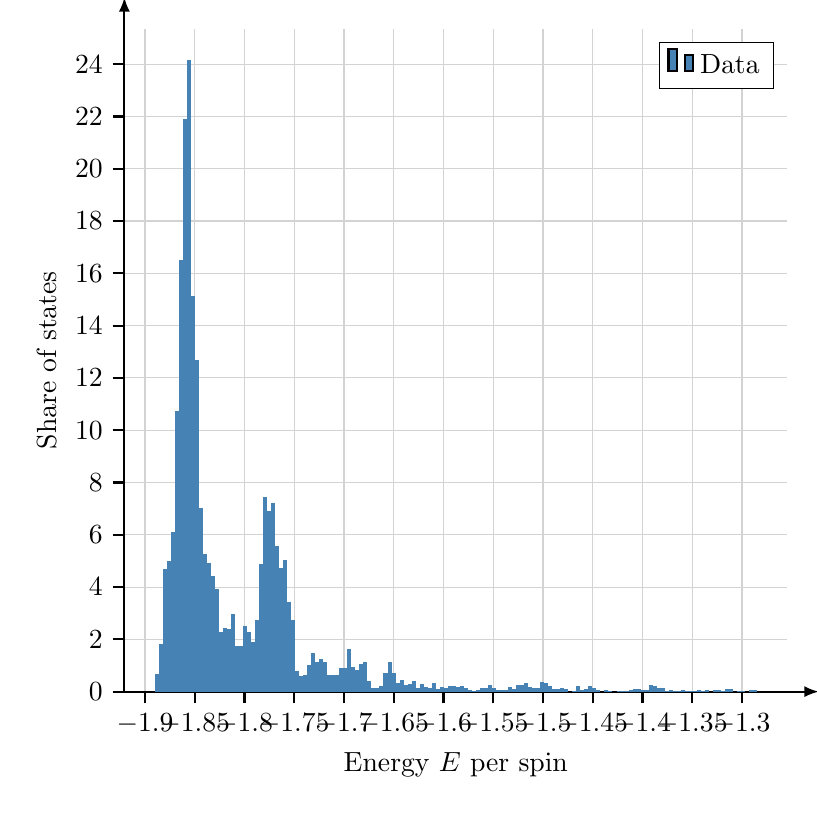
\begin{tikzpicture}

\definecolor{lightgray}{RGB}{211,211,211}
\definecolor{steelblue}{RGB}{70,130,180}

\begin{axis}[
tick align=outside,
tick pos=left,
x grid style={lightgray},
xlabel={Energy \(\displaystyle E\) per spin},
xmajorgrids,
xmin=-1.92068, xmax=-1.25452,
xtick style={color=black},
y grid style={lightgray},
ylabel={Share of states},
ymajorgrids,
ymin=0, ymax=25.353895123842,
ytick style={color=black}
]
\draw[draw=none,fill=steelblue] (axis cs:-1.8904,0) rectangle (axis cs:-1.88636266666667,0.669360680887585);
\addlegendimage{ybar,ybar legend,draw=none,fill=steelblue}
\addlegendentry{Data}

\draw[draw=none,fill=steelblue] (axis cs:-1.88636266666667,0) rectangle (axis cs:-1.88232533333333,1.83454408835847);
\draw[draw=none,fill=steelblue] (axis cs:-1.88232533333333,0) rectangle (axis cs:-1.878288,4.6855247662131);
\draw[draw=none,fill=steelblue] (axis cs:-1.878288,0) rectangle (axis cs:-1.87425066666667,5.00780953849203);
\draw[draw=none,fill=steelblue] (axis cs:-1.87425066666667,0) rectangle (axis cs:-1.87021333333333,6.09861953697578);
\draw[draw=none,fill=steelblue] (axis cs:-1.87021333333333,0) rectangle (axis cs:-1.866176,10.7345620305299);
\draw[draw=none,fill=steelblue] (axis cs:-1.866176,0) rectangle (axis cs:-1.86213866666667,16.5108967952271);
\draw[draw=none,fill=steelblue] (axis cs:-1.86213866666667,0) rectangle (axis cs:-1.85810133333333,21.8905733786558);
\draw[draw=none,fill=steelblue] (axis cs:-1.85810133333333,0) rectangle (axis cs:-1.854064,24.1465667846114);
\draw[draw=none,fill=steelblue] (axis cs:-1.854064,0) rectangle (axis cs:-1.85002666666667,15.1225931607928);
\draw[draw=none,fill=steelblue] (axis cs:-1.85002666666667,0) rectangle (axis cs:-1.84598933333333,12.6682706642058);
\draw[draw=none,fill=steelblue] (axis cs:-1.84598933333333,0) rectangle (axis cs:-1.841952,7.01589158115468);
\draw[draw=none,fill=steelblue] (axis cs:-1.841952,0) rectangle (axis cs:-1.83791466666667,5.255720901784);
\draw[draw=none,fill=steelblue] (axis cs:-1.83791466666667,0) rectangle (axis cs:-1.83387733333333,4.93343612950452);
\draw[draw=none,fill=steelblue] (axis cs:-1.83387733333333,0) rectangle (axis cs:-1.82984,4.4376134029214);
\draw[draw=none,fill=steelblue] (axis cs:-1.82984,0) rectangle (axis cs:-1.82580266666667,3.94179067633779);
\draw[draw=none,fill=steelblue] (axis cs:-1.82580266666667,0) rectangle (axis cs:-1.82176533333333,2.28078454228362);
\draw[draw=none,fill=steelblue] (axis cs:-1.82176533333333,0) rectangle (axis cs:-1.817728,2.42953136025851);
\draw[draw=none,fill=steelblue] (axis cs:-1.817728,0) rectangle (axis cs:-1.81369066666667,2.3799490876003);
\draw[draw=none,fill=steelblue] (axis cs:-1.81369066666667,0) rectangle (axis cs:-1.80965333333333,2.97493635950022);
\draw[draw=none,fill=steelblue] (axis cs:-1.80965333333333,0) rectangle (axis cs:-1.805616,1.76017067937106);
\draw[draw=none,fill=steelblue] (axis cs:-1.805616,0) rectangle (axis cs:-1.80157866666667,1.76017067937096);
\draw[draw=none,fill=steelblue] (axis cs:-1.80157866666667,0) rectangle (axis cs:-1.79754133333333,2.52869590557532);
\draw[draw=none,fill=steelblue] (axis cs:-1.79754133333333,0) rectangle (axis cs:-1.793504,2.2807845422835);
\draw[draw=none,fill=steelblue] (axis cs:-1.793504,0) rectangle (axis cs:-1.78946666666667,1.88412636101691);
\draw[draw=none,fill=steelblue] (axis cs:-1.78946666666667,0) rectangle (axis cs:-1.78542933333333,2.72702499620853);
\draw[draw=none,fill=steelblue] (axis cs:-1.78542933333333,0) rectangle (axis cs:-1.781392,4.88385385684646);
\draw[draw=none,fill=steelblue] (axis cs:-1.781392,0) rectangle (axis cs:-1.77735466666667,7.46213203507971);
\draw[draw=none,fill=steelblue] (axis cs:-1.77735466666667,0) rectangle (axis cs:-1.77331733333333,6.89193589950921);
\draw[draw=none,fill=steelblue] (axis cs:-1.77331733333333,0) rectangle (axis cs:-1.76928,7.21422067178802);
\draw[draw=none,fill=steelblue] (axis cs:-1.76928,0) rectangle (axis cs:-1.76524266666667,5.55321453773404);
\draw[draw=none,fill=steelblue] (axis cs:-1.76524266666667,0) rectangle (axis cs:-1.76120533333333,4.73510703887118);
\draw[draw=none,fill=steelblue] (axis cs:-1.76120533333333,0) rectangle (axis cs:-1.757168,5.03260067482148);
\draw[draw=none,fill=steelblue] (axis cs:-1.757168,0) rectangle (axis cs:-1.75313066666667,3.44596794975442);
\draw[draw=none,fill=steelblue] (axis cs:-1.75313066666667,0) rectangle (axis cs:-1.74909333333333,2.72702499620868);
\draw[draw=none,fill=steelblue] (axis cs:-1.74909333333333,0) rectangle (axis cs:-1.745056,0.793316362533391);
\draw[draw=none,fill=steelblue] (axis cs:-1.745056,0) rectangle (axis cs:-1.74101866666667,0.594987271900076);
\draw[draw=none,fill=steelblue] (axis cs:-1.74101866666667,0) rectangle (axis cs:-1.73698133333333,0.644569544558416);
\draw[draw=none,fill=steelblue] (axis cs:-1.73698133333333,0) rectangle (axis cs:-1.732944,1.01643658949591);
\draw[draw=none,fill=steelblue] (axis cs:-1.732944,0) rectangle (axis cs:-1.72890666666667,1.46267704342094);
\draw[draw=none,fill=steelblue] (axis cs:-1.72890666666667,0) rectangle (axis cs:-1.72486933333333,1.14039227114181);
\draw[draw=none,fill=steelblue] (axis cs:-1.72486933333333,0) rectangle (axis cs:-1.720832,1.23955681645849);
\draw[draw=none,fill=steelblue] (axis cs:-1.720832,0) rectangle (axis cs:-1.71679466666667,1.14039227114175);
\draw[draw=none,fill=steelblue] (axis cs:-1.71679466666667,0) rectangle (axis cs:-1.71275733333333,0.619778408229212);
\draw[draw=none,fill=steelblue] (axis cs:-1.71275733333333,0) rectangle (axis cs:-1.70872,0.644569544558416);
\draw[draw=none,fill=steelblue] (axis cs:-1.70872,0) rectangle (axis cs:-1.70468266666667,0.644569544558416);
\draw[draw=none,fill=steelblue] (axis cs:-1.70468266666667,0) rectangle (axis cs:-1.70064533333333,0.917272044179233);
\draw[draw=none,fill=steelblue] (axis cs:-1.70064533333333,0) rectangle (axis cs:-1.696608,0.892480907850065);
\draw[draw=none,fill=steelblue] (axis cs:-1.696608,0) rectangle (axis cs:-1.69257066666667,1.63621499772521);
\draw[draw=none,fill=steelblue] (axis cs:-1.69257066666667,0) rectangle (axis cs:-1.68853333333333,0.942063180508454);
\draw[draw=none,fill=steelblue] (axis cs:-1.68853333333333,0) rectangle (axis cs:-1.684496,0.842898635191728);
\draw[draw=none,fill=steelblue] (axis cs:-1.684496,0) rectangle (axis cs:-1.68045866666667,1.04122772582513);
\draw[draw=none,fill=steelblue] (axis cs:-1.68045866666667,0) rectangle (axis cs:-1.67642133333333,1.11560113481258);
\draw[draw=none,fill=steelblue] (axis cs:-1.67642133333333,0) rectangle (axis cs:-1.672384,0.396658181266717);
\draw[draw=none,fill=steelblue] (axis cs:-1.672384,0) rectangle (axis cs:-1.66834666666667,0.148746817975011);
\draw[draw=none,fill=steelblue] (axis cs:-1.66834666666667,0) rectangle (axis cs:-1.66430933333333,0.148746817975019);
\draw[draw=none,fill=steelblue] (axis cs:-1.66430933333333,0) rectangle (axis cs:-1.660272,0.198329090633348);
\draw[draw=none,fill=steelblue] (axis cs:-1.660272,0) rectangle (axis cs:-1.65623466666667,0.718942953545925);
\draw[draw=none,fill=steelblue] (axis cs:-1.65623466666667,0) rectangle (axis cs:-1.65219733333333,1.11560113481258);
\draw[draw=none,fill=steelblue] (axis cs:-1.65219733333333,0) rectangle (axis cs:-1.64816,0.718942953545925);
\draw[draw=none,fill=steelblue] (axis cs:-1.64816,0) rectangle (axis cs:-1.64412266666667,0.32228477227919);
\draw[draw=none,fill=steelblue] (axis cs:-1.64412266666667,0) rectangle (axis cs:-1.64008533333333,0.446240453925057);
\draw[draw=none,fill=steelblue] (axis cs:-1.64008533333333,0) rectangle (axis cs:-1.636048,0.272702499620853);
\draw[draw=none,fill=steelblue] (axis cs:-1.636048,0) rectangle (axis cs:-1.63201066666667,0.297493635950038);
\draw[draw=none,fill=steelblue] (axis cs:-1.63201066666667,0) rectangle (axis cs:-1.62797333333333,0.396658181266695);
\draw[draw=none,fill=steelblue] (axis cs:-1.62797333333333,0) rectangle (axis cs:-1.623936,0.148746817975019);
\draw[draw=none,fill=steelblue] (axis cs:-1.623936,0) rectangle (axis cs:-1.61989866666667,0.297493635950022);
\draw[draw=none,fill=steelblue] (axis cs:-1.61989866666667,0) rectangle (axis cs:-1.61586133333333,0.173537954304189);
\draw[draw=none,fill=steelblue] (axis cs:-1.61586133333333,0) rectangle (axis cs:-1.611824,0.148746817975011);
\draw[draw=none,fill=steelblue] (axis cs:-1.611824,0) rectangle (axis cs:-1.60778666666667,0.347075908608378);
\draw[draw=none,fill=steelblue] (axis cs:-1.60778666666667,0) rectangle (axis cs:-1.60374933333333,0.0991645453166739);
\draw[draw=none,fill=steelblue] (axis cs:-1.60374933333333,0) rectangle (axis cs:-1.599712,0.173537954304189);
\draw[draw=none,fill=steelblue] (axis cs:-1.599712,0) rectangle (axis cs:-1.59567466666667,0.148746817975011);
\draw[draw=none,fill=steelblue] (axis cs:-1.59567466666667,0) rectangle (axis cs:-1.59163733333333,0.223120226962528);
\draw[draw=none,fill=steelblue] (axis cs:-1.59163733333333,0) rectangle (axis cs:-1.5876,0.223120226962528);
\draw[draw=none,fill=steelblue] (axis cs:-1.5876,0) rectangle (axis cs:-1.58356266666667,0.173537954304179);
\draw[draw=none,fill=steelblue] (axis cs:-1.58356266666667,0) rectangle (axis cs:-1.57952533333333,0.198329090633348);
\draw[draw=none,fill=steelblue] (axis cs:-1.57952533333333,0) rectangle (axis cs:-1.575488,0.123955681645849);
\draw[draw=none,fill=steelblue] (axis cs:-1.575488,0) rectangle (axis cs:-1.57145066666667,0.0495822726583397);
\draw[draw=none,fill=steelblue] (axis cs:-1.57145066666667,0) rectangle (axis cs:-1.56741333333333,0.0247911363291685);
\draw[draw=none,fill=steelblue] (axis cs:-1.56741333333333,0) rectangle (axis cs:-1.563376,0.0743734089875054);
\draw[draw=none,fill=steelblue] (axis cs:-1.563376,0) rectangle (axis cs:-1.55933866666667,0.148746817975019);
\draw[draw=none,fill=steelblue] (axis cs:-1.55933866666667,0) rectangle (axis cs:-1.55530133333333,0.123955681645849);
\draw[draw=none,fill=steelblue] (axis cs:-1.55530133333333,0) rectangle (axis cs:-1.551264,0.272702499620853);
\draw[draw=none,fill=steelblue] (axis cs:-1.551264,0) rectangle (axis cs:-1.54722666666667,0.123955681645842);
\draw[draw=none,fill=steelblue] (axis cs:-1.54722666666667,0) rectangle (axis cs:-1.54318933333333,0.0743734089875095);
\draw[draw=none,fill=steelblue] (axis cs:-1.54318933333333,0) rectangle (axis cs:-1.539152,0.0495822726583397);
\draw[draw=none,fill=steelblue] (axis cs:-1.539152,0) rectangle (axis cs:-1.53511466666667,0.0743734089875054);
\draw[draw=none,fill=steelblue] (axis cs:-1.53511466666667,0) rectangle (axis cs:-1.53107733333333,0.173537954304179);
\draw[draw=none,fill=steelblue] (axis cs:-1.53107733333333,0) rectangle (axis cs:-1.52704,0.0991645453166793);
\draw[draw=none,fill=steelblue] (axis cs:-1.52704,0) rectangle (axis cs:-1.52300266666667,0.247911363291698);
\draw[draw=none,fill=steelblue] (axis cs:-1.52300266666667,0) rectangle (axis cs:-1.51896533333333,0.247911363291685);
\draw[draw=none,fill=steelblue] (axis cs:-1.51896533333333,0) rectangle (axis cs:-1.514928,0.347075908608359);
\draw[draw=none,fill=steelblue] (axis cs:-1.514928,0) rectangle (axis cs:-1.51089066666667,0.173537954304189);
\draw[draw=none,fill=steelblue] (axis cs:-1.51089066666667,0) rectangle (axis cs:-1.50685333333333,0.123955681645849);
\draw[draw=none,fill=steelblue] (axis cs:-1.50685333333333,0) rectangle (axis cs:-1.502816,0.123955681645842);
\draw[draw=none,fill=steelblue] (axis cs:-1.502816,0) rectangle (axis cs:-1.49877866666667,0.371867044937547);
\draw[draw=none,fill=steelblue] (axis cs:-1.49877866666667,0) rectangle (axis cs:-1.49474133333333,0.32228477227919);
\draw[draw=none,fill=steelblue] (axis cs:-1.49474133333333,0) rectangle (axis cs:-1.490704,0.223120226962528);
\draw[draw=none,fill=steelblue] (axis cs:-1.490704,0) rectangle (axis cs:-1.48666666666667,0.0991645453166739);
\draw[draw=none,fill=steelblue] (axis cs:-1.48666666666667,0) rectangle (axis cs:-1.48262933333333,0.0991645453166793);
\draw[draw=none,fill=steelblue] (axis cs:-1.48262933333333,0) rectangle (axis cs:-1.478592,0.123955681645842);
\draw[draw=none,fill=steelblue] (axis cs:-1.478592,0) rectangle (axis cs:-1.47455466666667,0.0991645453166793);
\draw[draw=none,fill=steelblue] (axis cs:-1.47455466666667,0) rectangle (axis cs:-1.47051733333333,0);
\draw[draw=none,fill=steelblue] (axis cs:-1.47051733333333,0) rectangle (axis cs:-1.46648,0.0247911363291698);
\draw[draw=none,fill=steelblue] (axis cs:-1.46648,0) rectangle (axis cs:-1.46244266666667,0.198329090633348);
\draw[draw=none,fill=steelblue] (axis cs:-1.46244266666667,0) rectangle (axis cs:-1.45840533333333,0.0495822726583397);
\draw[draw=none,fill=steelblue] (axis cs:-1.45840533333333,0) rectangle (axis cs:-1.454368,0.0991645453166739);
\draw[draw=none,fill=steelblue] (axis cs:-1.454368,0) rectangle (axis cs:-1.45033066666667,0.198329090633359);
\draw[draw=none,fill=steelblue] (axis cs:-1.45033066666667,0) rectangle (axis cs:-1.44629333333333,0.123955681645842);
\draw[draw=none,fill=steelblue] (axis cs:-1.44629333333333,0) rectangle (axis cs:-1.442256,0.0495822726583397);
\draw[draw=none,fill=steelblue] (axis cs:-1.442256,0) rectangle (axis cs:-1.43821866666667,0);
\draw[draw=none,fill=steelblue] (axis cs:-1.43821866666667,0) rectangle (axis cs:-1.43418133333333,0.0495822726583397);
\draw[draw=none,fill=steelblue] (axis cs:-1.43418133333333,0) rectangle (axis cs:-1.430144,0.0247911363291685);
\draw[draw=none,fill=steelblue] (axis cs:-1.430144,0) rectangle (axis cs:-1.42610666666667,0);
\draw[draw=none,fill=steelblue] (axis cs:-1.42610666666667,0) rectangle (axis cs:-1.42206933333333,0.0247911363291685);
\draw[draw=none,fill=steelblue] (axis cs:-1.42206933333333,0) rectangle (axis cs:-1.418032,0.0247911363291698);
\draw[draw=none,fill=steelblue] (axis cs:-1.418032,0) rectangle (axis cs:-1.41399466666667,0.0247911363291685);
\draw[draw=none,fill=steelblue] (axis cs:-1.41399466666667,0) rectangle (axis cs:-1.40995733333333,0.0743734089875095);
\draw[draw=none,fill=steelblue] (axis cs:-1.40995733333333,0) rectangle (axis cs:-1.40592,0.0991645453166793);
\draw[draw=none,fill=steelblue] (axis cs:-1.40592,0) rectangle (axis cs:-1.40188266666667,0.0991645453166739);
\draw[draw=none,fill=steelblue] (axis cs:-1.40188266666667,0) rectangle (axis cs:-1.39784533333333,0.0495822726583369);
\draw[draw=none,fill=steelblue] (axis cs:-1.39784533333333,0) rectangle (axis cs:-1.393808,0.0495822726583397);
\draw[draw=none,fill=steelblue] (axis cs:-1.393808,0) rectangle (axis cs:-1.38977066666667,0.247911363291698);
\draw[draw=none,fill=steelblue] (axis cs:-1.38977066666667,0) rectangle (axis cs:-1.38573333333333,0.198329090633348);
\draw[draw=none,fill=steelblue] (axis cs:-1.38573333333333,0) rectangle (axis cs:-1.381696,0.148746817975011);
\draw[draw=none,fill=steelblue] (axis cs:-1.381696,0) rectangle (axis cs:-1.37765866666667,0.148746817975019);
\draw[draw=none,fill=steelblue] (axis cs:-1.37765866666667,0) rectangle (axis cs:-1.37362133333333,0.0247911363291698);
\draw[draw=none,fill=steelblue] (axis cs:-1.37362133333333,0) rectangle (axis cs:-1.369584,0.0743734089875054);
\draw[draw=none,fill=steelblue] (axis cs:-1.369584,0) rectangle (axis cs:-1.36554666666667,0.0247911363291685);
\draw[draw=none,fill=steelblue] (axis cs:-1.36554666666667,0) rectangle (axis cs:-1.36150933333333,0.0247911363291698);
\draw[draw=none,fill=steelblue] (axis cs:-1.36150933333333,0) rectangle (axis cs:-1.357472,0.0743734089875095);
\draw[draw=none,fill=steelblue] (axis cs:-1.357472,0) rectangle (axis cs:-1.35343466666667,0.0247911363291685);
\draw[draw=none,fill=steelblue] (axis cs:-1.35343466666667,0) rectangle (axis cs:-1.34939733333333,0.0247911363291685);
\draw[draw=none,fill=steelblue] (axis cs:-1.34939733333333,0) rectangle (axis cs:-1.34536,0.0247911363291698);
\draw[draw=none,fill=steelblue] (axis cs:-1.34536,0) rectangle (axis cs:-1.34132266666667,0.0495822726583397);
\draw[draw=none,fill=steelblue] (axis cs:-1.34132266666667,0) rectangle (axis cs:-1.33728533333333,0.0247911363291685);
\draw[draw=none,fill=steelblue] (axis cs:-1.33728533333333,0) rectangle (axis cs:-1.333248,0.0495822726583369);
\draw[draw=none,fill=steelblue] (axis cs:-1.333248,0) rectangle (axis cs:-1.32921066666667,0);
\draw[draw=none,fill=steelblue] (axis cs:-1.32921066666667,0) rectangle (axis cs:-1.32517333333333,0.0495822726583397);
\draw[draw=none,fill=steelblue] (axis cs:-1.32517333333333,0) rectangle (axis cs:-1.321136,0.0495822726583369);
\draw[draw=none,fill=steelblue] (axis cs:-1.321136,0) rectangle (axis cs:-1.31709866666667,0.0247911363291685);
\draw[draw=none,fill=steelblue] (axis cs:-1.31709866666667,0) rectangle (axis cs:-1.31306133333333,0.0991645453166793);
\draw[draw=none,fill=steelblue] (axis cs:-1.31306133333333,0) rectangle (axis cs:-1.309024,0.0991645453166793);
\draw[draw=none,fill=steelblue] (axis cs:-1.309024,0) rectangle (axis cs:-1.30498666666667,0);
\draw[draw=none,fill=steelblue] (axis cs:-1.30498666666667,0) rectangle (axis cs:-1.30094933333333,0.0247911363291685);
\draw[draw=none,fill=steelblue] (axis cs:-1.30094933333333,0) rectangle (axis cs:-1.296912,0.0247911363291698);
\draw[draw=none,fill=steelblue] (axis cs:-1.296912,0) rectangle (axis cs:-1.29287466666667,0);
\draw[draw=none,fill=steelblue] (axis cs:-1.29287466666667,0) rectangle (axis cs:-1.28883733333333,0.0495822726583369);
\draw[draw=none,fill=steelblue] (axis cs:-1.28883733333333,0) rectangle (axis cs:-1.2848,0.0495822726583397);
\end{axis}

\end{tikzpicture}

\end{figure}

\begin{figure}
\centering
\graphicspath{{../../Plots/}}
% This file was created with tikzplotlib v0.10.1.
\begin{tikzpicture}

\definecolor{darkgray176}{RGB}{176,176,176}

\begin{axis}[
tick align=outside,
tick pos=left,
x grid style={darkgray176},
xmin=-0.5, xmax=19.5,
xtick style={color=black},
y dir=reverse,
y grid style={darkgray176},
ymin=-0.5, ymax=19.5,
ytick style={color=black}
]
\addplot graphics [includegraphics cmd=\pgfimage,xmin=-0.5, xmax=19.5, ymin=19.5, ymax=-0.5] {High_temp_state_10000-001.png};
\end{axis}

\end{tikzpicture}

\end{figure}

\begin{figure}
\centering
\graphicspath{{../../Plots/}}
\input{../../Plots/Medium_temp_state_10000.pgf}
\end{figure}

\begin{figure}
\centering
\graphicspath{{../../Plots/}}
% This file was created with tikzplotlib v0.10.1.
\begin{tikzpicture}

\definecolor{lightgray}{RGB}{211,211,211}

\begin{axis}[
tick align=outside,
tick pos=left,
x grid style={lightgray},
xmajorgrids,
xmin=-0.5, xmax=19.5,
xtick style={color=black},
y dir=reverse,
y grid style={lightgray},
ymajorgrids,
ymin=-0.5, ymax=19.5,
ytick style={color=black}
]
\addplot graphics [includegraphics cmd=\pgfimage,xmin=-0.5, xmax=19.5, ymin=19.5, ymax=-0.5] {../../Plots/Low_temp_state_10000-002.png};
\end{axis}

\end{tikzpicture}

\end{figure}


\newpage
\section*{Bibliography}
%\nocite{*}
%Main source
%\printbibliography[heading=none, keyword={main}]
%\noindent Other sources
\printbibliography[heading=none, keyword={secondary}]

\end{document}
